\documentclass{article}
\usepackage{luatextra}
\usepackage{polyglossia}
\usepackage{ulem}
\usepackage{framed}
\usepackage{color}
\usepackage{geometry}
\usepackage{amsmath}
\usepackage{unicode-math}
\usepackage[hidelinks]{hyperref}
\usepackage{latexsym}
\usepackage{pdflscape}
\usepackage{pdfpages}
\usepackage{enumitem}
\usepackage{titlesec}
\usepackage{lastpage}
\usepackage{fancyhdr}
\usepackage{titlesec}
\usepackage{listings}
\usepackage{graphicx}
\usepackage{float}
\usepackage{pdfpages}
\usepackage{ccicons}
\usepackage{array}
\usepackage{listings}

\usepackage{ifluatex}
\ifluatex
  \usepackage{pdftexcmds}
  \makeatletter
  \let\pdfstrcmp\pdf@strcmp
  \let\pdffilemoddate\pdf@filemoddate
  \makeatother
\fi
\usepackage{svg}

\setmathfont{xits-math.otf}

\setmainlanguage{french}
\selectlanguage{french}
%%\setmainfont{Latin Modern Roman}
\setmainfont{Roboto}

\geometry{margin={1in,1in}}

\setlist{nosep} %% No space between lists' items

\pagestyle{fancy}
\fancyhead[R]{}

%% <current page>/<total pages> footer
\cfoot{\thepage/\pageref{LastPage}}

\newcommand\image[2]{
\directlua{
local image = img.scan({filename = "#1"})

image.height = image.height * #2
image.width  = image.width  * #2

node.write(img.node(image))
}
}


%%%%%%%%%%%%%%%%%%%%%%%%%%%%%%%%%%%%%%%%%%
%% \subsubsubsection command definition %%
%%%%%%%%%%%%%%%%%%%%%%%%%%%%%%%%%%%%%%%%%%


\titleclass{\subsubsubsection}{straight}[\subsection]

\newcounter{subsubsubsection}[subsubsection]
\renewcommand\thesubsubsubsection{\thesubsubsection.\arabic{subsubsubsection}}
\renewcommand\theparagraph{\thesubsubsubsection.\arabic{paragraph}} % optional; useful if paragraphs are to be numbered

\titleformat{\subsubsubsection}
  {\normalfont\normalsize\bfseries}{\thesubsubsubsection}{1em}{}
\titlespacing*{\subsubsubsection}
{0pt}{3.25ex plus 1ex minus .2ex}{1.5ex plus .2ex}

\makeatletter
\renewcommand\paragraph{\@startsection{paragraph}{5}{\z@}%
  {3.25ex \@plus1ex \@minus.2ex}%
  {-1em}%
  {\normalfont\normalsize\bfseries}}
\renewcommand\subparagraph{\@startsection{subparagraph}{6}{\parindent}%
  {3.25ex \@plus1ex \@minus .2ex}%
  {-1em}%
  {\normalfont\normalsize\bfseries}}
\def\toclevel@subsubsubsection{4}
\def\toclevel@paragraph{5}
\def\toclevel@paragraph{6}
\def\l@subsubsubsection{\@dottedtocline{4}{7em}{4em}}
\def\l@paragraph{\@dottedtocline{5}{10em}{5em}}
\def\l@subparagraph{\@dottedtocline{6}{14em}{6em}}
\makeatother

\setcounter{secnumdepth}{4}
\setcounter{tocdepth}{4}

%%%%%%%%%%%%%%%%%%%%%%%%%%%%%%%%%%%%%%%%%%
%% end \subsubsubsection definition     %%
%%%%%%%%%%%%%%%%%%%%%%%%%%%%%%%%%%%%%%%%%%


\titlespacing*{\section}{0pt}{0.7\baselineskip}{0.7\baselineskip}

\title{Projet Principe d'éxécution des programmes}
%\subtitle{Meow}
\author{NassimBounouas, piernov}
\date{\today}

\begin{document}
\lstset{xleftmargin=.25in}

\maketitle
\textcolor{blue}{\url{https://github.com/NassimBounouas/Stage_SI3_PeP}}
\tableofcontents

\newpage

\documentclass{article}

\usepackage{../parm}
\begin{document}

    \section{Présentation du projet}

    \subsection{Le microprocesseur ARM Cortex-M0}

    La famille des ARM Cortex-M regroupe des processeurs 32 bits.
    Ils peuvent être utilisés comme microprocesseur ou microcontrôleur.
    On les retrouve dans diverses applications : Arduino Due, machine à laver, distributeur de boissons... Les Cortex-M visent en majorité le marché de l'embarqué.

    Le but de ce projet est de simuler le comportement d'un Cortex-M0 au moyen d'un logiciel de simulation électronique: Logisim.
    L'idée est ici d'obtenir un système ayant un comportement similaire à un Cortex-M0 et non une copie conforme du fait de la complexité d'un processeur réel.

    \subsection{Le projet}
    Durant ce projet nous allons implémenter notre microprocesseur en le divisant en plusieurs blocs:
    \begin{itemize}
        \item Partie matérielle:
        \begin{itemize}
            \item ALU 32 bits
            \item Banc de 8 registres
            \item Contrôleur
        \end{itemize}
        \item Partie logicielle:
        \begin{itemize}
            \item Assembleur
            \item Exportation sur FPGA
        \end{itemize}
    \end{itemize}

    \paragraph{Spécificités de l'implémentation}
    \begin{itemize}
        \item Pas de gestion des interruptions
        \item Pas de gestion des appels de fonctions
        \item Pas d'optimisation
        \item Pas de pipeline
        \item Pas de FPU \footnote{\textit{Floating-Point Unit}, unité de calcul en virgule flottante}
        \item Pas de MMU \footnote{\textit{Memory Management Unit}, unité de gestion mémoire, gère la traduction des adresses virtuelles en adresses physiques au sein du processeur}
        \item Toutes les instructions s'exécutent en 1 cycle (excepté les instructions \texttt{LDR}/\texttt{STR} en 2 cycles)
        \item Instructions sur 16 bits
        \item Données sur 32 bits
        \item Adressage RAM/ROM sur 9 bits
        \item Adressage RAM uniquement sur la pile (en utilisant le \textit{Stack Pointer})
    \end{itemize}

    \subsection{Logisim}

    Logisim est un programme permettant la modélisation et la simulation de circuit logique.
    La modélisation du circuit ne se fait que par dessin et glisser-déposer des différents éléments électroniques.

    \paragraph{Installation:} la version de Logisim utilisé dans le cadre du projet est la 3.5.0, accessible à l'adresse \url{https://github.com/logisim-evolution/logisim-evolution/releases/tag/v3.5.0}.
    Sur Windows, utilisez le fichier \texttt{.msi} pour installer.
    sur Mac, utilisez le fichier \texttt{.dmg}.
    Sur Ubuntu/Debian, passez par le fichier \texttt{.deb} avec la commande :
    \begin{lstlisting}
sudo apt install gdebi
sudo gdebi logisim-evolution_3.5.0-1_amd64.deb
    \end{lstlisting}
    Pour les autres systèmes, vous pouvez lancer directement le fichier .jar sans installer.

    \textit{Cette section est un extrait du tutoriel officiel «Introduction à l’utilisation de Logisim». Pour plus d'informations, se référer à la documentation officielle.}

    Vous pouvez voir l'interface de Logisim sur la Figure  \ref{fig_logisim_description}.

    \begin{figure}[t]
        \begin{center}
            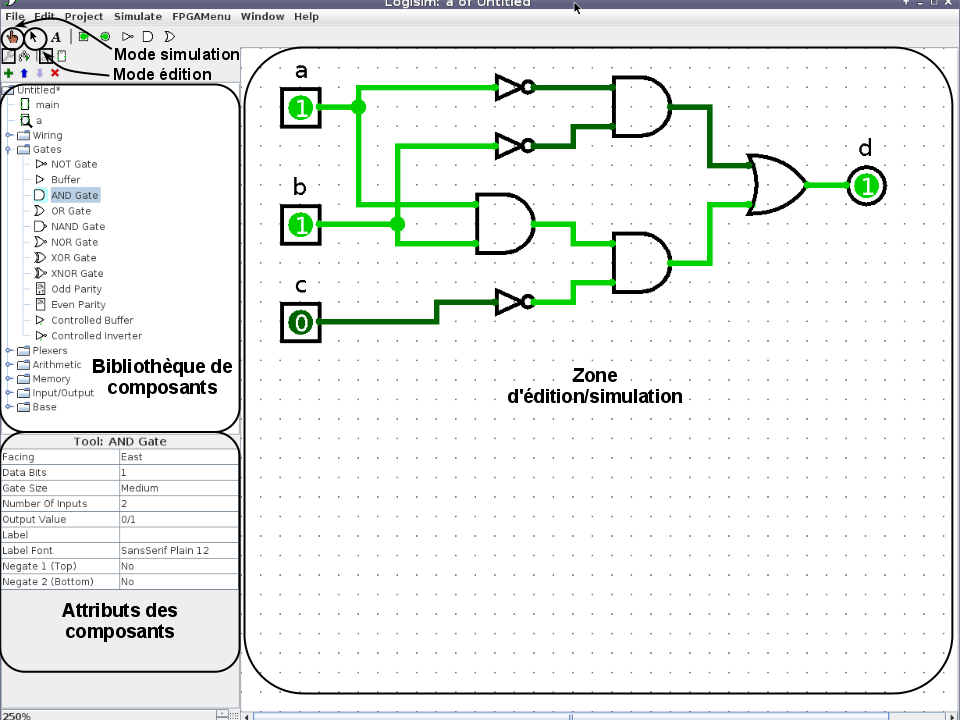
\includegraphics[width=500pt]{pictures/Logisim_description.png}
            \caption{\label{fig_logisim_description}Interface de Logisim}
        \end{center}
    \end{figure}

    Une des particularités de \texttt{Logisim} est de pouvoir éditer et simuler un circuit en même temps.
    Nous expliquerons plus tard dans ce document comment simuler un circuit, puis comment l'implémenter sur la carte du
    laboratoire.


%%%%%%%%%%%%%%%%%%%%%%%%%%%%%%%%%%%%%%%%%%%%%%%%%

    \subsubsection{Mode édition}
    \begin{enumerate}
        \item Pour utiliser le mode édition, il faut simplement sélectionner la flèche comme indiqué en haut de la figure
        \ref{fig_logisim_description}.
        \item On peut alors choisir un composant dans la bibliothèque sur la gauche.
        Pour l'ajouter dans son schéma, il suffit
        de cliquer sur le composant désiré, puis de cliquer sur le schéma.

        \item Chaque composant que vous utiliserez aura des attributs modifiables dans la zone inférieur gauche de
        \texttt{Logisim}.
        Par exemple si l'on pose une porte \texttt{AND}, on peut modifier le nombre de signaux qu'elle prend en
        entrée, ou encore mettre un inverseur sur une de ses entrées.

        \item Il est aussi possible de faire des copier/coller d'un ou plusieurs composants.
        Dans ce cas, les composants
        conserverons aussi tous les attributs préalablement définis.

        \item Une fois que l'on a posé tous les composants, il faut alors les connecter.
        Pour cela il suffit de placer le curseur
        avec la souris sur un des ports à connecter et, en gardant pressé le bouton
        gauche de la souris, le déplacer jusqu'au port de destination.

    \end{enumerate}

%%%%%%%%%%%%%%%%%%%%%%%%%%%%%%%%%%%%%%%%%%%%%%%%%

    \subsubsection{Création d'un premier circuit}



    \label{nouveauCircuit}
    Tous les circuits réalisés dans \texttt{Logisim} peuvent être réutilisés dans d'autres circuits.
    Afin de créer un nouveau circuit, il faut aller dans \texttt{Projet} $\rightarrow$ \texttt{Ajouter Circuit...} et nommer le circuit.
    Le circuit créé devient un composant disponible dans la bibliothèque.

%%%%%%%%%%%%%%%%%%%%%%%%%%%%%%%%%%%%%%%%%%%%%%%%%

    \subsubsection{Mode simulation}
    \texttt{Logisim} est capable de simuler le circuit en affichant les valeurs des signaux directement sur le schéma.
    L'utilisateur
    peut alors définir les valeurs des bits en entrée et observer la réaction du design.
    \begin{enumerate}
        \item Pour utiliser le mode simulation, il faut sélectionner la main en haut à gauche de \texttt{Logisim} (cf
        Figure~\ref{fig_logisim_description})

        \item Il est alors possible de contrôler l'état des différentes entrées en cliquant directement dessus.

        \item En cliquant sur une entrée, la valeur doit alterner entre \texttt{0} ou \texttt{1}.

        \item Voici un descriptif des couleurs utilisées pour les signaux en mode simulation.
        \begin{figure}[H]
            \begin{center}
                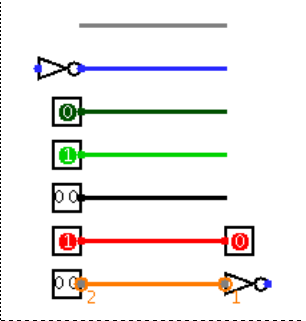
\includegraphics[scale=0.4]{pictures/logisim_couleurs.png}
                \caption{\label{fig_logisim_couleur}Couleurs des fils en simulation}
            \end{center}
        \end{figure}

        \begin{itemize}
            \item \textbf{Gris}: La taille du fil est inconnue.
            Le fil n'est relié à aucune entrée ou sortie.
            \item \textbf{Bleu}: Le fil comporte une valeur, cependant elle est inconnue.
            \item \textbf{Vert foncé}: Le fil comporte la valeur \texttt{0}.
            \item \textbf{Vert clair}: Le fil comporte la valeur \texttt{1}.
            \item \textbf{Noir}: Le fil comporte plusieurs bits (bus).
            \item \textbf{Rouge}: Le fil comporte une erreur.
            \item \textbf{Orange}: Les composants reliés au fil n'ont pas la bonne taille.
        \end{itemize}

    \end{enumerate}

%%%%%%%%%%%%%%%%%%%%%%%%%%%%%%%%%%%%%%%%%%%%%%%%%

    \subsubsection{Design hiérarchique}
    La méthodologie de design que l'on vient d'utiliser est valable pour la conception de systèmes numériques plutôt
    simples, c'est-à-dire avec un nombre de portes logiques plutôt bas.
    Lorsque l'on vise des systèmes plus compliqués on
    risque de voir le nombre de portes et de connexions exploser.
    Dans ce cas, le risque d'introduire des erreurs devient
    très important.

    La clé pour gérer correctement une complexité plus grande est d'utiliser le design hiérarchique.
    Grâce au design
    hiérarchique on peut travailler à différents niveaux d'abstraction.
    D'abord on décrit des blocs de base à l'aide des
    portes logiques, pour ensuite utiliser ces blocs de base comme parties d'un système plus large.

    Pour créer un design hiérarchique il faudra suivre les pas
    suivants:
    \begin{enumerate}
        \item Créez un nouveau circuit comme déjà expliqué dans la section \ref{nouveauCircuit} et nommez le.
        Pour passer de l'édition d'un circuit à l'autre, il suffit de double-cliquer sur le nom de celui désiré dans le menu de
        gauche.
        \item Il est alors possible d'ajouter un sous circuit de la même manière que l'utilisation d'un
        composant quelconque.
        On clique sur le sous circuit en question dans le menu indiqué sur la Figure~\ref{fig_sousCircuit}, puis on le
        place en cliquant sur la zone d'édition.
        \item Si le sous circuit avait été créé correctement, alors il devrait être représenté par un petit bloc, avec
        sur sa gauche des points bleus correspondant aux entrées et sur sa droite des points verts correspondant aux sorties.
        \item Si les sorties apparaissent en bleu et non en vert sur le schéma, vérifiez que vous avez bien affecté l'attribut
        \texttt{Sortie?} $=$ \texttt{Oui} dans les \texttt{Pin}s de sortie.

    \end{enumerate}

    \begin{figure}[H]
        \begin{center}
            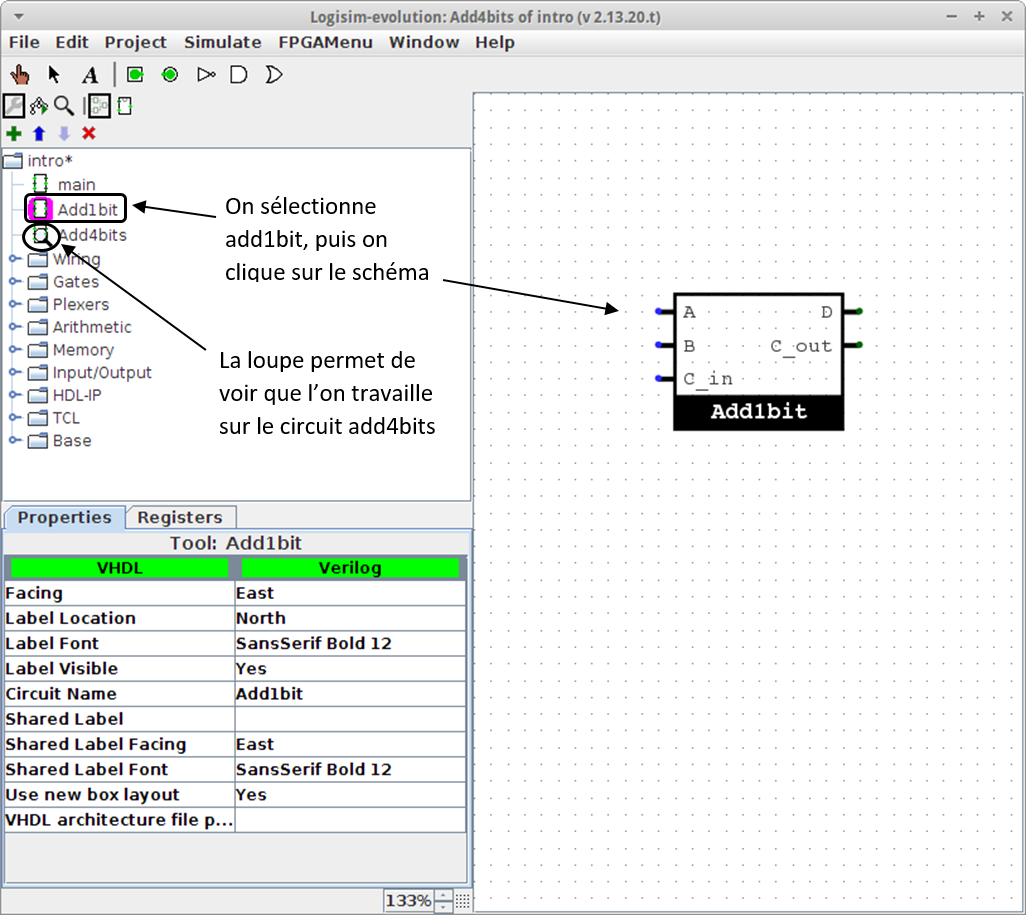
\includegraphics[width=450pt]{pictures/logisim_sousCircuit.png}
            \caption{\label{fig_sousCircuit}Sous circuit}
        \end{center}
    \end{figure}

    \subsubsection{Bus et séparateurs}

    Pour l'implémentation de composant travaillant avec des données sur plusieurs bits (un additionneur par exemple),
    il devient nécessaire de regrouper plusieurs signaux en créant un bus de données.
    Par exemple, pour définir l'entrée A comme un bus de 4 bits, il
    faut ajouter un élément \texttt{Pin} et définir sa taille via l'attribut \texttt{Data bits} $=$ \texttt{4}.

    \paragraph{}
    Lorsque l'on tire un fil de l'une de ces entrées, ce n'est plus un simple signal mais un bus de 4 bits.
    Pour
    pouvoir connecter les éléments de ce bus aux entrées de plusieurs composants travaillant sur chacun un bit,
    on va devoir séparer les différents fils du bus afin de pouvoir les traiter un par un.
    L'élément \texttt{Séparateur}
    de \texttt{Cablage} permet d'effectuer ces conversions dans les deux sens: d'un bus de 4 bits vers 4 fils,
    et de 4 fils vers un bus de 4 bits -- voir Figure~\ref{fig_splitter}.

    \begin{figure}[H]
        \begin{center}
            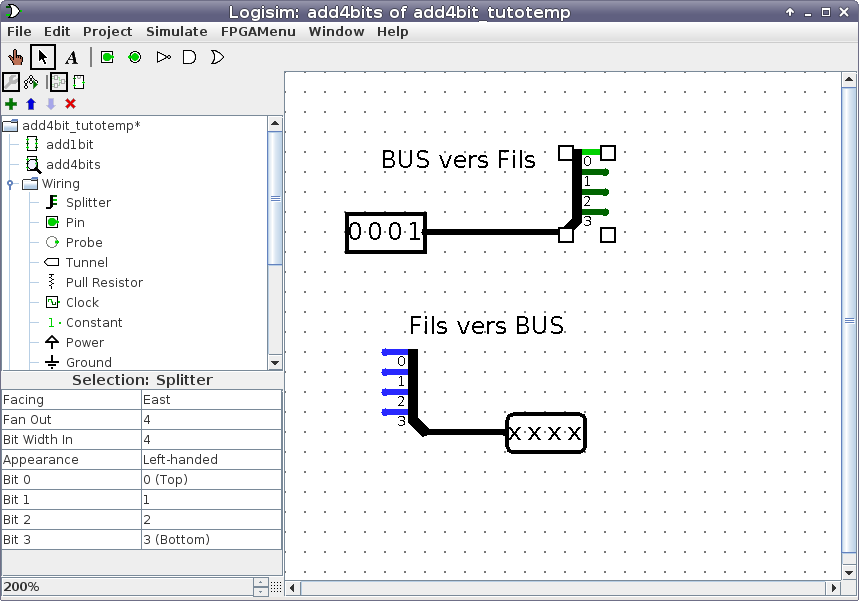
\includegraphics[width=500pt]{pictures/logisim_splitters.png}
            \caption{\label{fig_splitter}Exemples splitters}
        \end{center}
    \end{figure}

    Il faut définir les tailles d'entrées et de sorties du \texttt{Séparateur} via les attributs \texttt{Ventilation en sortie} et
    \texttt{Largeur de bits en entrée}.

    \paragraph{Note:} le bit de poids faible est indexé à 0 en sortie du \texttt{splitter}.

    \paragraph{Remarque:} n'utiliser que des composants dont l'indicateur \texttt{VHDL} dans la zone \texttt{Properties} est vert.
    Les autres (\texttt{Buffer controllé} par exemple) ne pourront pas être déployés sur la carte FPGA.
\end{document}
\section{Décodeur 7 segment}
\subsection{Introduction}
Nous allons commencer par une prise en main de logisim en réalisant un décodeur 7 segments. Ce type d'afficheur est un grand classique en ce qui concerne l'affichage de caractères hexadécimaux.

Le principe de cet afficheur est très simple, En allumant plusieurs segments en même temps nous allons pouvoir représenter les caractères suivants :
0,1,2,3,4,5,6,7,8,9,A,B,C,D,E,F.

\begin{center}
        \makebox[\textwidth]{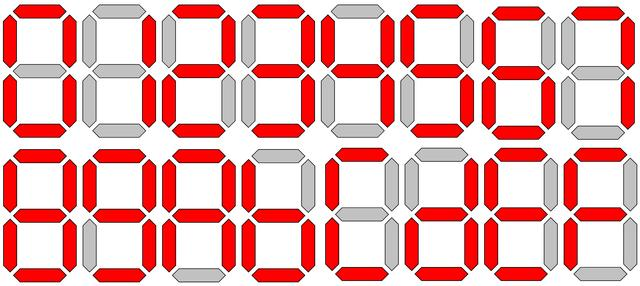
\includegraphics[width=15cm]{pictures/7seg.jpg}}
\end{center}

\subsubsection{meow}
miaounyanmeowmjau


\section{Organisation du travail}

\paragraph{}
	Afin de répartir au mieux le travail 4 ou 5 sous-tâches sont indiquées selon la taille du groupe.

\subsection{ALU (Matériel)}

\begin{itemize}
	\item Réaliser les blocs d'opérateurs arithmétiques et logiques
	\item Générer les flags
\end{itemize}

\subsection{Contrôleur (Matériel)}

\begin{itemize}
	\item Lecture des instructions depuis la mémoire de programme 
	\item Décodage de l'instruction et génération des signaux de commande du chemin de données
	\item Calcul de l'adresse de la prochaine instruction
\end{itemize}

\subsection{Chemin de données (Matériel)}

\begin{itemize}
	\item Mouvement de registre à registre
 	\item Lecture mémoire des données
	\item Ecriture mémoire des données
	\item Envoie d'adresse pour la lecture et l'écriture
\end{itemize}

\subsection{Assembleur (Logiciel)}

\begin{itemize}
	\item Parser un fichier assembleur 
	\item Générer le fichier binaire à charger dans la mémoire d'instruction de logisim
\end{itemize}

\subsection{FPGA (Logiciel) (groupe de 5)}

\begin{itemize}
	\item Tester le déploiement du processeur sur FPGA 
\end{itemize}

\documentclass{article}

\usepackage{../parm}
\begin{document}

    \section{ALU}
    \label{sec:ALU}

    \subsection{Description}

    L'unité arithmétique et logique est l'élèment qui se charge des calculs au sein du processeur.
    Les ALU les plus basiques ne font que des opérations sur des entiers cependant on trouve des ALU spécialisées.
    Les calculs sur ces dernières vont des opérations à virgule flottante jusqu'à des calculs plus complexes tels que des racines carrées, des logarithmes, des sinus ou cosinus... Notre ALU n'effectuera que des calculs simples (addition, soustraction, multiplication, décalage) sur des entiers de 32 bits.

    Une ALU comporte deux entrées amenant les données à traiter.
    Une troisième entrée permet de désigner le calcul à effectuer.
    En sortie on retrouvera le résultat de l'opération ainsi que des drapeaux.
    Ces drapeaux représentent une série d'état à la suite d'un calcul : un résultat négatif, un résultat nul, un débordement ou encore une retenue.

    L'entrée \texttt{Shift} indique le nombre de décalage pour les opérations de décalage.

    \paragraph{Remarque:} les instructions \texttt{TST}, \texttt{CMP}, \texttt{CMN} n'enregistrent pas le résultat de l'opération.
    Seuls les drapeaux sont mis à jour.
    Pour ces opérations en particulier, il faudra recopier l'entrée \texttt{B} sur la sortie \texttt{S}.
    Le contrôleur définira le même registre pour le registre \texttt{Rn} d'opérande B que pour le registre \texttt{Rd} de destination de la sortie S.

    \paragraph{Remarque 2:} pour l'instruction \texttt{SBC}, la retenue entrante doit être inversée (voir \textit{\ref{subsubsubsec:SBC}~\nameref{subsubsubsec:SBC}}).

    \subsection{Interface}

    \subsubsection{Entrées}

    \begin{tabular}{|l|r|l|}
        \hline
        \textbf{Port}   & \textbf{Taille} & \textbf{Description} \\
        \hline

        \texttt{A}      & \texttt{32}     & Première opérande    \\
        \hline
        \texttt{B}      & \texttt{32}     & Seconde opérande     \\
        \hline
        \texttt{Shift}  & \texttt{5}      & Nombre de décalage   \\
        \hline
        \texttt{CarryIn} & \texttt{1}      & Retenu entrente      \\
        \hline
        \texttt{Codop}  & \texttt{4}      & Code opération ALU   \\

        \hline
    \end{tabular}

    \subsubsection{Sorties}

    \begin{tabular}{|l|r|l|}
        \hline
        \textbf{Port}   & \textbf{Taille} & \textbf{Description}                    \\
        \hline

        \texttt{S}     & \texttt{32}     & Registre résultat                       \\
        \hline
        \texttt{Flags} & \texttt{4}      & Registre drapeaux, ordre: \texttt{NZCV} \\

        \hline
    \end{tabular}

    \subsection{Opérations}
    \label{subsec:Opcodes}
    Ces opérations de l'ALU correspondent exactement aux instructions de la catégorie \textit{Data Processing}.
    En cas de doute, se référer à \textit{\ref{sec:ISA}~\nameref{sec:ISA}}.

    \begin{tabular}{|r|c|l|l|}
        \hline
        \textbf{Codop} & \textbf{Opération}            & \textbf{Instructions} & \textbf{Remarque}                                  \\
        \hline

        $0000$         & \texttt{A and B}            & AND                &                                                    \\
        \hline
        $0001$         & \texttt{A xor B}            & EOR                &                                                    \\
        \hline
        $0010$         & \texttt{B << Shift}         & LSL                & Retenue sortante, voir jeu d'instructions           \\
        \hline
        $0011$         & \texttt{B >> Shift}         & LSR                & Retenue sortante, voir jeu d'instructions           \\
        \hline
        $0100$         & \texttt{B >> Shift (arith)}  & ASR                & Retenue sortante, voir jeu d'instructions           \\
        \hline
        $0101$         & \texttt{A + B + CarryIn}     & ADC                &                                                    \\
        \hline
        $0110$         & \texttt{B – A + CarryIn – 1} & SBC                & Retenue entrante inversée                          \\
        \hline
        $0111$         & \texttt{B >> Shift (rot)}    & ROR                & Retenue sortante, voir jeu d'instructions           \\
        \hline
        $1000$         & \texttt{A and B}            & TST                & Résultat perdu, seuls les drapeaux sont mis à jour \\
        \hline
        $1001$         & \texttt{–A}                & RSB                & Registre Rm utilisé plutôt que Rn                  \\
        \hline
        $1010$         & \texttt{B – A}             & CMP                & Résultat perdu, seuls les drapeaux sont mis à jour \\
        \hline
        $1011$         & \texttt{A + B}             & CMN                & Résultat perdu, seuls les drapeaux sont mis à jour \\
        \hline
        $1100$         & \texttt{A or B}             & ORR                &                                                    \\
        \hline
        $1101$         & \texttt{A * B}             & MUL                &                                                    \\
        \hline
        $1110$         & \texttt{B and not A}        & BIC                &                                                    \\
        \hline
        $1111$         & \texttt{not B}             & MVN                &  Complément binaire \\
        \hline
    \end{tabular}

    \subsection{Drapeaux}

    Ces drapeaux de l'ALU correspondent exactement aux drapeaux de l'architecture ARM. En cas de doute, se référer à \textit{\ref{sec:ISA}~\nameref{sec:ISA}} et \textit{\ref{subsec:Flags}~\nameref{subsec:Flags}} .

    \begin{tabular}{|c|l|l|}
        \hline
        \textbf{Symbole} & \textbf{Nom}       & \textbf{Description}                                 \\
        \hline

        \texttt{N}      & \texttt{Negative} & Résultat négatif                                     \\
        \hline
        \texttt{Z}      & \texttt{Zero}    & Résultat nul                                         \\
        \hline
        \texttt{C}      & \texttt{CarryOut} & Retenue sortante (dépassement de capacité non-signé). \\
        \hline
        \texttt{V}      & \texttt{Overflow} & Dépassement de capacité signé                        \\

        \hline
    \end{tabular}
\end{document}

\section{Banc de registres}

\subsection{Description}

	\paragraph{}
	Le processeur ne stocke pas le résultat d'un calcul directement en RAM, pour cela il travaille avec une mémoire rapide mais petite constituée de quelques registres (20 registres de 32 bits un dans Cortex-M0).

	\paragraph{}
	Parmi les 20 registres présents dans un Cortex-M0, seuls 13 d'entre eux sont dédiés à un usage général. Les 7 autres ont un usage bien particulier (voir tableau suivant)

\vspace{1em}

\begin{tabular}{|c|c|c|c|c|}
\hline
\textbf{Nom} 	 & \textbf{Accès}              & \textbf{Valeur de remise à zéro} & \textbf{Description} & \textbf{A implémenter}\\
\hline
\texttt{R0 - R12} &  \texttt{LE} &  \texttt{Inconnue}		  &  \texttt{Registres à usage général} &  \texttt{ OUI (uniquement 8)}\\
\hline
\texttt{MSP} 	 &  \texttt{LE} &  \texttt{?} 			  &  \texttt{Pointeur de pile} &  \texttt{ Oui (contrôleur)}\\
\hline
\texttt{PSP}	 &  \texttt{LE} &  \texttt{Inconnue} 		  &  \texttt{Pointeur de pile} &  \texttt{Oui (contrôleur)}\\
\hline
\texttt{LR} 	 &  \texttt{LE} &  \texttt{Inconnue} 		  &  \texttt{Registre de lien} &  \texttt{Non}\\
\hline
\texttt{PC} 	 &  \texttt{LE} &  \texttt{?} 			  &  \texttt{Compteur d'instruction} &  \texttt{Oui (contrôleur)}\\
\hline
\texttt{PSR} 	 &  \texttt{LE} &  \texttt{Inconnue} 		  &  \texttt{Statut du programme} &  \texttt{Non}\\
\hline
\texttt{ASPSR} 	 &  \texttt{LE} &  \texttt{Inconnue} 		  &  \texttt{Statut d'application du programme} &  \texttt{Non}\\
\hline
\texttt{IPSR} 	 &  \texttt{L}      &  \texttt{0x00000000} 		  &  \texttt{Statut d'interruption du programme} &  \texttt{Non}\\
\hline
\texttt{EPSR} 	 &  \texttt{L}      &  \texttt{Inconnue} 		  &  \texttt{Statut d'exécution du programme} &  \texttt{Non}\\
\hline
\texttt{PRIMASK}  &  \texttt{LE} &  \texttt{0x00000000} 		  &  \texttt{Masque de priorité} &  \texttt{Non}\\
\hline
\texttt{CONTROL}  &  \texttt{LE} &  \texttt{0x00000000} 		  &  \texttt{Registre de contrôle} &  \texttt{Non}\\
\hline
\end{tabular}

\paragraph{}
Dans notre cas, le banc de registre ne contient que 8 registres \texttt{R0-R7} par soucis de simplicité. Les registres \texttt{PC} et \texttt{SP} sont implémentés dans le contrôleur.



\subsection{Interface}

\subsubsection{Entrées}

\begin{tabular}{|l|r|l|}
\hline
\textbf{Port}		& \textbf{Taille} & \textbf{Description}\\
\hline

\texttt{DataIn}		& \texttt{32} & Données entrantes, à enregistrer dans le registre sélectionné\\
\hline
\texttt{RegDest}	&  \texttt{3} & Sélection du registre de destination des données entrantes\\
\hline
\texttt{Clk}		&  \texttt{1} & Horloge\\
\hline
\texttt{Reset}		&  \texttt{1} & Remise à zéro\\
\hline
\texttt{RegA}		&  \texttt{3} & Sélection du registre A pour les données sortantes\\
\hline
\texttt{RegB}		&  \texttt{3} & Sélection du registre B pour les données sortantes\\

\hline
\end{tabular}


\subsubsection{Sorties}

\begin{tabular}{|l|r|l|}
\hline 
\textbf{Port} & \textbf{Taille} & \textbf{Description}\\
\hline

\texttt{AOut}	& \texttt{32} & Données sortantes du registre sélectionné A\\
\hline
\texttt{BOut}	& \texttt{32} & Données sortantes du registre sélectionné B\\
\hline
\texttt{R0}	& \texttt{32} & Registre interne 0\\
\hline
\texttt{R1}	& \texttt{32} & Registre interne 1\\
\hline
\texttt{R2}	& \texttt{32} & Registre interne 2\\
\hline
\texttt{R3}	& \texttt{32} & Registre interne 3\\
\hline
\texttt{R4}	& \texttt{32} & Registre interne 4\\
\hline
\texttt{R5}	& \texttt{32} & Registre interne 5\\
\hline
\texttt{R6}	& \texttt{32} & Registre interne 6\\
\hline
\texttt{R7}	& \texttt{32} & Registre interne 7\\

\hline
\end{tabular}

Les sorties \texttt{R0-R7} ne seront pas utilisées pour implémenter une quelconque fonctionalité. Elles sont présentes pour aider à visualiser le comportement du processeur.

\subsection{Interaction avec l'ALU}

Après avoir réalisé l'ALU et le banc de registres, l'interaction entre ces composants peut être mise en oeuvre de la manière suivante:

\hspace{14em}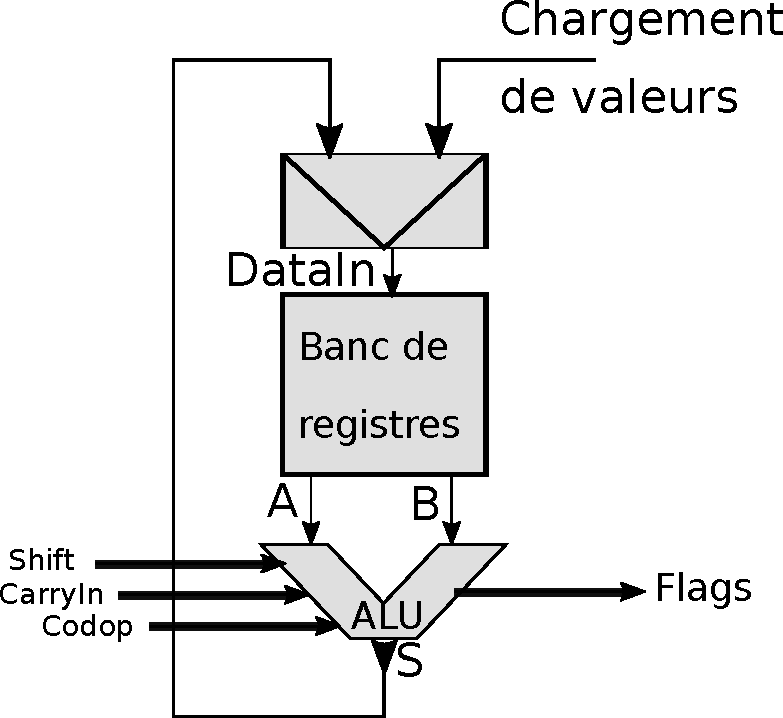
\includegraphics[scale=0.5]{pictures/ALU_Registers.pdf}

Il est ainsi possible de valider leur comportement en enregistrant des données dans le banc de registre (à l'aide des ports \texttt{DataIn} et \texttt{RegDest})
puis en effectuant diverses opération par l'ALU en spécifiant  le \texttt{Codop}.

\documentclass{article}

\usepackage{../parm}

\begin{document}

    \section{Contrôleur}

    \subsection{Description}

    Le contrôleur ou unité de contrôle (Control unit en anglais) joue le rôle de chef d'orchestre au sein du processeur.
    Il est en charge du décodage des instructions.
    En fonction des informations récupérées au sein de l'instruction et des différents drapeaux, le contrôleur va agir sur le chemin de données.

    Il est responsable du choix de la source fournissant les données.
    La sortie \texttt{Load} selon si elle est à 0 ou à 1 choisira respectivement un chargement depuis l'ALU ou directement depuis la RAM.
    Le même mécanisme est utilisé pour choisir la source du nombre de décalage, des immédiats 8 (voir tableau des sorties).

    Le contrôleur abrite de plus le compteur ordinal et l'incrémente lorsqu'il traite une instruction.

    \subsection{Interface}

    \subsubsection{Entrées}

    \begin{tabular}{|l|r|l|}
        \hline
        \textbf{Port}  & \textbf{Taille} & \textbf{Description}                    \\
        \hline

        \texttt{Inst}  & \texttt{16}     & Instruction à traiter                   \\
        \hline
        \texttt{Flags} & \texttt{4}      & Drapeaux en entrée, ordre \texttt{NZCV} \\
        \hline
        \texttt{Clk}   & \texttt{1}      & Horloge                                 \\
        \hline
        \texttt{Reset} & \texttt{1}      & Remise à Zero                           \\
        \hline


        \hline
    \end{tabular}

    \subsubsection{Sorties}

    \begin{tabular}{|l|r|l|}
        \hline
        \textbf{Port}          & \textbf{Taille} & \textbf{Description}                                                                               \\
        \hline

        \hline
        \texttt{Carry}         & \texttt{1}      & Retenue sortante (provenant des drapeaux) à destination de l'ALU                                   \\
        \hline
        \texttt{DP\_Shift}     & \texttt{1}      & Provenance du nombre de décalage: 0 pour registre A, 1 pour Imm5                                  \\
        \hline
        \texttt{Imm32\_Enable} & \texttt{1}      & Provenance de la donnée A: 0 pour registre, 1 pour Imm32                                           \\
        \hline
        \texttt{Imm5}          & \texttt{5}      & Nombre de décalage pour les instructions de décalage de la catégorie \textit{Shift, add, sub, mov} \\
        \hline
        \texttt{Imm32}         & \texttt{8}      & Valeur pour les instructions \texttt{MOV}, \texttt{CMP}, \texttt{ADD} et \texttt{SUB}    \\
        \hline
        \texttt{ALU\_Opcode}   & \texttt{4}      & Code opération à destination de l'ALU                                                              \\
        \hline
        \texttt{Rm}            & \texttt{3}      & Séléction du registre pour lecture de l'opérande A                                                 \\
        \hline
        \texttt{Rn}            & \texttt{3}      & Sélection du registre pour lecture de l'opérande B                                                 \\
        \hline
        \texttt{Rd}            & \texttt{3}      & Sélection du registre pour enregistrement du résultat                                              \\
        \hline
        \texttt{RAM\_Addr}     & \texttt{32}     & Adresse mémoire des instructions \textit{Load/Store}                                               \\
        \hline
        \texttt{Load}          & \texttt{1}      & Provenance des données en entrée du banc de registre                                               \\
        \hline
        \texttt{Store}         & \texttt{1}      & 1 pour stocker la valeur du registre \texttt{Rm} à l'adresse \texttt{RAM\_Address}                  \\
        \hline
        \texttt{PC}            & \texttt{16}      & Compteur ordinal: adresse de la prochaine instruction en ROM                                       \\
        \hline
        \texttt{Flags}         & \texttt{4}      & Valeur des drapeaux issue de Flags APSR                \\
        \hline
        
        \texttt{SP}            & \texttt{32}     & Valeur de SP                                                                                       \\
        \hline
    \end{tabular}

    \subsection{Sous composants}

    \subsubsection{Décodeur d'instruction}
    \label{sec:OpDec}

    \subsubsubsection{Description}

    Le bloc \textit{Opcode Decoder} active l'une de ses sorties en fonction de la catégorie d'instruction reconnue, afin d'activer les blocs correspondant du contrôleur.

    L'entrée \texttt{Opcode} correspond au code opération pré-extrait de l'instruction, c'est à dire les 6 bits de poids fort de l'instruction.

    Les sorties doivent être activées en fonction du code binaire correspondant à chacune d'elle.
    Voir \textit{\ref{sec:ISA}~\nameref{sec:ISA}}.

    \subsubsubsection{Interface}

    \textbf{Entrées}\\

    \begin{tabular}{|l|r|l|}
        \hline
        \textbf{Port}   & \textbf{Taille} & \textbf{Description}     \\
        \hline

        \texttt{Opcode} & \texttt{6}      & Code opération à décoder \\

        \hline
    \end{tabular}

    \vspace{1em}
    \textbf{Sorties}\\

    \begin{tabular}{|l|r|l|}
        \hline
        \textbf{Port}             & \textbf{Taille} & \textbf{Description}                         \\
        \hline

        \texttt{Shift}            & \texttt{1}      & Active le bloc \textit{Shift, add, sub, mov} \\
        \hline
        \texttt{Data\_Processing} & \texttt{1}      & Active le bloc \textit{Data Processing}      \\
        \hline
        \texttt{Load\_Store}      & \texttt{1}      & Active le bloc \textit{Load/Store}           \\
        \hline
        \texttt{SP\_Address}      & \texttt{1}      & Active le bloc \textit{SP Address}           \\
        \hline
        \texttt{Branch}           & \texttt{1}      & Active le bloc \textit{Conditional}          \\

        \hline
    \end{tabular}

    \subsubsection{Shift, add, sub, mov}
    \label{sec:SASM}
    \subsubsubsection{Description}

    Le bloc \textit{Shift, add, sub, mov} traite les instructions de calcul de la catégorie \texttt{Shift, add, sub, mov} (voir \textit{\ref{subsubsec:ShiftAddSubMov}~\nameref{subsubsec:ShiftAddSubMov}}).

    La sortie \texttt{ALU\_Opcode} devra être définie pour chacune des instructions afin d'exécuter la bonne opération dans l'ALU (voir \textit{\ref{subsec:Opcodes}~\nameref{subsec:Opcodes}}).

    Certaines instructions ne mettent pas à jour tous les drapeaux.
    La sortie \texttt{Flags\_Update\_Mask} doit être définie en conséquence avec le masque dont les bits à 1 correspondent aux drapeaux à mettre à jour.

    La sortie \texttt{Carry} force la valeur de la retenue entrante pour l'ALU. Les instructions \texttt{ADD} et \texttt{SUB} n'utilisent pas de retenue entrante.
    Elle doit être définie à 0 pour \texttt{ADD} et à 1 pour \texttt{SUB} étant donnée qu'elle est est inversée pour la soustraction dans l'ALU.

    La sortie \texttt{Imm32} est utilisée pour communiquer les valeurs des immédiats de \texttt{MOV}, \texttt{CMP}, \texttt{ADD} et \texttt{SUB} à l'ALU. Dans ce cas, la sortie \texttt{Imm32\_Enable} doit être définie à 1.
    Les immédiats devront être étendus de 3 ou 8 bits vers 32 bits en complétant par des zéros (ce sont des entiers non-signés).

    La sortie \texttt{Imm5} est utilisée en tant que valeur du nombre de décalage pour les instructions de décalage \texttt{LSL}, \texttt{LSR} et \texttt{ASR}.

    Si l'entrée \texttt{Enable} est à 0, les sorties sont forcées à 0.

    \paragraph{Remarque:} l'immédiat pour l'instruction \texttt{MOV} passe par l'ALU pour être enregistré dans le registre de destination.
    Pour que la valeur ne soit pas modifiée, on peut l'inverser ici et utiliser l'opération \texttt{RSB} dans l'ALU.

    \paragraph{Remarque 2:} pour les opérations de décalage, on préfèrera utiliser le registre \texttt{Rn} à la place de \texttt{Rm} pour rester cohérent avec les instructions de la catégorie \textit{Data Processing}.
    L'ALU travaillera uniquement sur l'opérande B.

    \paragraph{Remarque 3:} quand une instruction ne fait pas usage de certaines sorties, elles doivent être définies à 0.


    \subsubsubsection{Interface}

    \textbf{Entrées}\\

    \begin{tabular}{|l|r|l|}
        \hline
        \textbf{Port}        & \textbf{Taille} & \textbf{Description}                                \\
        \hline

        \texttt{Instruction} & \texttt{16}     & Instruction \textit{Shift, add, sub, mov} à décoder \\
        \hline
        \texttt{Enable} & \texttt{1} & Active le composant.
        Si 0, les sortie sont forcées à 0 \\


        \hline
    \end{tabular}

    \vspace{1em}
    \textbf{Sorties}\\

    \begin{tabular}{|l|r|l|}
        \hline
        \textbf{Port}                & \textbf{Taille} & \textbf{Description}                                                         \\
        \hline

        \texttt{ALU\_Opcode}         & \texttt{4}      & Code opération à destination de l'ALU                                        \\
        \hline
        \texttt{Rm}                  & \texttt{3}      & Sélection du registre opérande A                                             \\
        \hline
        \texttt{Rn}                  & \texttt{3}      & Sélection du registre opérande B                                             \\
        \hline
        \texttt{Rd}                  & \texttt{3}      & Sélection du registre résultat                                               \\
        \hline
        \texttt{Flags\_Update\_Mask} & \texttt{4}      & Masque de mise à jour des drapeaux à destination du bloc \textit{Flags APSR} \\
        \hline
        \texttt{Carry}               & \texttt{1}      & Valeur à utiliser en tant que retenue entrante pour l'ALU                    \\
        \hline
        \texttt{Imm32\_Enable}       & \texttt{1}      & Indique au processeur d'utiliser la sortie Imm32 à la place du registre Rm   \\
        \hline
        \texttt{Imm5}                & \texttt{5}      & Nombre de décalage à destination de l'ALU                                    \\
        \hline
        \texttt{Imm32}               & \texttt{32}     & Valeur à utiliser en tant qu'opérande A de l'ALU                             \\

        \hline
    \end{tabular}

    \subsubsection{Data Processing}
    \label{sec:DataProc}
    \subsubsubsection{Description}

    Le bloc \textit{Data Processing} traite les instructions de calcul de la catégorie \texttt{Data Processing} (voir \textit{\ref{subsubsec:DataProc}~\nameref{subsubsec:DataProc}}).

    La sortie \texttt{ALU\_Opcode} correspond aux bits 6 à 9, les code opérations de l'ALU ayant été implémenté en conséquence.

    Certaines instructions ne mettent pas à jour tous les drapeaux.
    La sortie \texttt{Flags\_Update\_Mask} doit être définie en conséquence avec le masque dont les bits à 1 correspondent aux drapeaux à mettre à jour.

    Si l'entrée \texttt{Enable} est à 0, les sorties sont forcées à 0.

    \paragraph{Remarque:} les instructions \texttt{TST}, \texttt{CMP} et \texttt{CMN} ne mettent à jour que les drapeaux et n'enregistrent pas le résultat de l'opération.
    Pour celles-ci, le registre \texttt{Rd} sera défini à \texttt{Rn} afin d'être cohérent avec les autres instructions, et que l'ALU puisse copier le contenu de l'opérande B dans le résultat.

    \paragraph{Remarque 2:} pour les instructions \texttt{RSB} et \texttt{MUL}, les bits 3 à 5 définissent le registre \texttt{Rn}, contrairement aux autres instructions pour lesquelles ces bits définissent le registre \texttt{Rm}.
    Pour simplifier l'implémentation du contrôleur, on considèrera toujours que les bits 3 à 5 correspondent à \texttt{Rm} et que les bits 0 à 2 correspondent à \texttt{Rdn}.
    Pour \texttt{RSB}, l'ALU devra alors faire usage de l'opérande \texttt{A} (en provenance du registre \texttt{Rm}).


    \subsubsubsection{Interface}

    \textbf{Entrées}\\

    \begin{tabular}{|l|r|l|}
        \hline
        \textbf{Port}        & \textbf{Taille} & \textbf{Description}                           \\
        \hline

        \texttt{Instruction} & \texttt{16}     & Instruction \textit{Data Processing} à décoder \\
        \hline
        \texttt{Enable} & \texttt{1} & Active le composant.
        Si 0, les sortie sont forcées à 0 \\


        \hline
    \end{tabular}

    \vspace{1em}
    \textbf{Sorties}\\

    \begin{tabular}{|l|r|l|}
        \hline
        \textbf{Port}                & \textbf{Taille} & \textbf{Description}                                                         \\
        \hline

        \texttt{ALU\_Opcode}         & \texttt{4}      & Code opération à destination de l'ALU                                        \\
        \hline
        \texttt{Rm}                  & \texttt{3}      & Sélection du registre opérande A                                             \\
        \hline
        \texttt{Rn}                  & \texttt{3}      & Sélection du registre opérande B                                             \\
        \hline
        \texttt{Rd}                  & \texttt{3}      & Sélection du registre résultat                                               \\
        \hline
        \texttt{Flags\_Update\_Mask} & \texttt{4}      & Masque de mise à jour des drapeaux à destination du bloc \textit{Flags APSR} \\

        \hline
    \end{tabular}

    \subsubsection{Flags APSR}
    \label{sec:FlagsAPSR}
    \subsubsubsection{Description}


    Le bloc \textit{Flags APSR} correspond au 4 bits de poids fort du registre \texttt{Application Program Status Register} de l'architecture ARM. Il conserve les drapeaux générés par la dernière instruction, afin qu'ils soient disponibles pour la prochaine instruction.

    L'entrée \texttt{Update\_Mask} permet de réinjecter l'ancien état d'un drapeau si le bit correspondant est à 0.
    Si le bit est à 1, le drapeau est mis à jour.

    \subsubsubsection{Interface}

    \textbf{Entrées}\\

    \begin{tabular}{|l|r|l|}
        \hline
        \textbf{Port}         & \textbf{Taille} & \textbf{Description}                                                      \\
        \hline

        \texttt{Flags\_In}    & \texttt{4}      & Nouveaux drapeaux générés par l'instruction courante, ordre \texttt{NZCV} \\
        \hline
        \texttt{Update\_Mask} & \texttt{4}      & Masque d'enregistrement des drapeaux, ordre \texttt{NZCV}                 \\
        \hline
        \texttt{Clk}          & \texttt{1}      & Horloge                                                                   \\
        \hline
        \texttt{Reset}        & \texttt{1}      & Remise à zéro                                                             \\


        \hline
    \end{tabular}

    \vspace{1em}
    \textbf{Sorties}\\

    \begin{tabular}{|l|r|l|}
        \hline
        \textbf{Port}       & \textbf{Taille} & \textbf{Description}                                               \\
        \hline

        \texttt{Flags\_Out} & \texttt{4}      & Drapeaux générés par l'instruction précédente, ordre \texttt{NZCV} \\

        \hline
    \end{tabular}

    \subsubsection{Load/Store}
    \label{sec:LoadStore}
    \subsubsubsection{Description}

    Le bloc \textit{Load/Store} traite les instructions de lecture/écriture en mémoire (voir \textit{\ref{subsubsec:LoadStore}~\nameref{subsubsec:LoadStore}}).

    La sortie \texttt{RAM\_Addr} correspond à l'adresse mémoire à laquelle effectuer l'opération.
    Elle est calculée en fonction de la valeur actuelle du \texttt{Stack\_Pointer} et de l'offset provenant de l'instruction.

    La sortie \texttt{Store} indique à la mémoire de stocker la donnée du registre Rm à l'adresse \texttt{RAM\_Addr}.
    La donnée sera écrite au cycle suivant.

    La sortie \texttt{Load} indique au processeur de présenter la donnée à l'adresse \texttt{RAM\_Addr} en entrée du banc de registre (\texttt{DataIn}).
    La donnée sera disponible au cycle suivant.

    La sortie \texttt{PC\_Hold} retarde l'incrémentation du \textit{Program Counter} d'un coup d'horloge.
    La RAM étant synchrone, elle a besoin d'un cycle pour traiter l'opération de lecture.
    La donnée lue n'est donc pas disponible immédiatement, et le processeur ne peut pas commencer à exécuter l'instruction suivante.
    La sortie \texttt{Load} devra donc elle aussi être retardée d'un cycle.

    Si l'entrée \texttt{Enable} est à 0, les sorties sont forcées à 0.

    \paragraph{Astuce:} utiliser une bascule D pour activer \texttt{PC\_Hold} et retarder \texttt{Load}.
    
	Pour vous aider, voici un chronogramme du comportement attendu : \\
    
\definecolor{bgblue}{rgb}{0.41961,0.80784,0.80784}%
\definecolor{bgred}{rgb}{1,0.61569,0.61569}%
\definecolor{fgblue}{rgb}{0,0,0.6}%
\definecolor{fgred}{rgb}{0.6,0,0}%
	\begin{tikztimingtable}[
    timing/slope=0,         % no slope
    timing/coldist=2pt,     % column distance
    xscale=4.05,yscale=1.1, % scale diagrams
    semithick               % set line width
  ]
  \scriptsize clock     & 7{C}                              \\
  Load                     &          LLHHLLH       \\
  PC\_Hold &          HHLLHHL       \\
  Store                     & [fgred]  HHHHHHH                  \\
\extracode
 \makeatletter
 \begin{pgfonlayer}{background}
  % Draw shaded backgrounds
  \shade [right color=bgblue,left color=white]
     (7,-4.45) rectangle (-2,-0.6);
  \shade [right color=bgred,left color=white]
     (7,-6.8) rectangle (-2,-4.6);
  % Add background grid lines
  \begin{scope}[gray,semitransparent,semithick]
    \horlines{}
    \foreach \x in {1,...,6}
      \draw (\x,1) -- (\x,-6.8);
    % similar: \vertlines{1,...,6}
  \end{scope}
  % Add labels
  \node [anchor=south east,inner sep=0pt]
    at (7,-4.45) {\tiny instruction LDR};
  \node [anchor=south east,inner sep=0pt,fgred]
    at (7,-6.8) {\tiny instruction STR};
 \end{pgfonlayer}
\end{tikztimingtable}

    \subsubsubsection{Interface}

    \textbf{Entrées}\\

    \begin{tabular}{|l|r|l|}
        \hline
        \textbf{Port}           & \textbf{Taille} & \textbf{Description}                                 \\
        \hline

        \texttt{Instruction}    & \texttt{16}     & Instruction de lecture/écriture en mémoire à décoder \\
        \hline
        \texttt{Enable} & \texttt{1} & Active le composant.
        Si 0, les sortie sont forcées à 0 \\
        \hline
        \texttt{Stack\_Pointer} & \texttt{32}     & Valeur courante du pointeur de pile                  \\
        \hline
        \texttt{Clk}            & \texttt{1}      & Horloge                                              \\
        \hline
        \texttt{Reset}          & \texttt{1}      & Remise à zéro                                        \\


        \hline
    \end{tabular}

    \vspace{1em}
    \textbf{Sorties}\\

    \begin{tabular}{|l|r|l|}
        \hline
        \textbf{Port}      & \textbf{Taille} & \textbf{Description}                                    \\
        \hline

        \texttt{Store}     & \texttt{1}      & Informe d'une opération d'écriture                      \\
        \hline
        \texttt{Load}      & \texttt{1}      & Informe d'une opération de lecture                      \\
        \hline
        \texttt{PC\_Hold}  & \texttt{1}      & Retarde l'incrémentation du compteur ordinal d'un cycle \\
        \hline
        \texttt{Rm}        & \texttt{3}      & Registre de provenance de la donnée écrite en mémoire   \\
        \hline
        \texttt{Rd}        & \texttt{3}      & Registre de destination de la donnée lue en mémoire     \\
        \hline
        \texttt{RAM\_Addr} & \texttt{32}     & Adresse mémoire à laquelle effectuer les opérations     \\

        \hline
    \end{tabular}

    \subsubsection{SP Address}
    \label{sec:SPAddr}
    \subsubsubsection{Description}

    Le bloc \textit{SP Address} traite les instructions de mise à jour du pointeur de pile (voir \textit{\ref{subsubsec:MiscInstr}~\nameref{subsubsec:MiscInstr}}).

    La sortie \texttt{New\_Stack\_Pointer} correspond à la nouvelle valeur du pointeur de pile qui sera enregistré dans le \textit{Stack Pointer}.
    Elle est calculée en fonction de la valeur actuelle du \texttt{Stack\_Pointer} et de l'opération en provenance de l'instruction (addition ou soustraction d'un immédiat).

    Si l'entrée \texttt{Enable} est à 0, la sortie \texttt{Write\_Enable} est forcée à 0.

    \subsubsubsection{Interface}

    \textbf{Entrées}\\

    \begin{tabular}{|l|r|l|}
        \hline
        \textbf{Port}           & \textbf{Taille} & \textbf{Description}                                     \\
        \hline

        \texttt{Instruction}    & \texttt{16}     & Instruction de mise à jour du pointeur de pile à décoder \\
        \hline
        \texttt{Enable} & \texttt{1} & Active le composant.
        Si 0, les sortie sont forcées à 0 \\
        \hline
        \texttt{Stack\_Pointer} & \texttt{32}     & Valeur courante du pointeur de pile                      \\

        \hline
    \end{tabular}

    \vspace{1em}
    \textbf{Sorties}\\

    \begin{tabular}{|l|r|l|}
        \hline
        \textbf{Port}                & \textbf{Taille} & \textbf{Description}                                                                        \\
        \hline

        \hline
        \texttt{Write\_Enable}       & \texttt{1}      & Le registre du pointeur de pile sera mis à jour avec la valeur \texttt{New\_Stack\_Pointer} \\
        \hline
        \texttt{New\_Stack\_Pointer} & \texttt{32}     & Nouvelle valeur du pointeur de pile                                                         \\

        \hline
    \end{tabular}

    \subsubsection{Conditional}
    \label{sec:Conditional}
    \subsubsubsection{Description}

    Le bloc conditionnel traite les instructions de branchement (voir \textit{\ref{subsubsec:Branching}~\nameref{subsubsec:Branching}}).

    Il vérifie éventuellement la condition à l'aide des drapeaux du registre \textit{Flags APSR}, selon le tableau  \textit{\ref{subsec:CondFlags}~\nameref{subsec:CondFlags}}.
    Si la condition est vérifiée, la sortie \texttt{Verified} passe à 1.

    La sortie \texttt{Offset} correspond à l'offset qui sera ajouté au \textit{Program Counter}, en provenance de l'instruction.

    Si l'entrée \texttt{Enable} est à 0, la sortie \texttt{Verified} est forcée à 0.

    \subsubsubsection{Interface}

    \textbf{Entrées}\\

    \begin{tabular}{|l|r|l|}
        \hline
        \textbf{Port}        & \textbf{Taille} & \textbf{Description}                              \\
        \hline

        \texttt{Instruction} & \texttt{16}     & Instruction du branchement conditionnel à décoder \\
        \hline
        \texttt{Enable} & \texttt{1} & Active le composant.
        Si 0, les sortie sont forcées à 0 \\
        \hline
        \texttt{N}           & \texttt{1}      & Drapeau négatif                                   \\
        \hline
        \texttt{Z}           & \texttt{1}      & Drapeau nul                                       \\
        \hline
        \texttt{C}           & \texttt{1}      & Drapeau retenue                                   \\
        \hline
        \texttt{V}           & \texttt{1}      & Drapeau dépassement de capacité                   \\


        \hline
    \end{tabular}

    \vspace{1em}
    \textbf{Sorties}\\

    \begin{tabular}{|l|r|l|}
        \hline
        \textbf{Port}     & \textbf{Taille} & \textbf{Description}                                               \\

        \hline
        \texttt{Verified} & \texttt{1}      & La condition est vérifiée                                          \\
        \hline
        \texttt{Offset}   & \texttt{8}      & Offset à appliquer au Program Counter si la condition est vérifiée \\

        \hline
    \end{tabular}

    \subsubsection{Program Counter}

    \subsubsubsection{Description}

    Le compteur ordinal (\textit{Program Counter}), aussi appelé pointeur d'instruction (\textit{Instruction Pointer}),
    est un compteur 16 bits dont la valeur donne l'adresse de la prochaine instruction à exécuter.
    Il est déjà implémenté directement dans le contrôleur.

    Il s'incrémente automatiquement à chaque front descendant d'horloge lorsque le signal \texttt{Count} est à l'état haut.
    Le signal \texttt{PC\_Hold} sortant du sous-composant \textit{Load/Store} retarde cette incrémentation d'un cycle afin de laisser le temps à la RAM de présenter la donnée sélectionnée sur sa sortie.
    En effet, étant synchrone, elle n'agit qu'au coup d'horloge suivant.

    Lorsque le signal \texttt{Load} est à l'état haut, le compteur charge la valeur suivante à partir de son entrée au prochain coup d'horloge.
    Les instructions de branchement (voir \textit{\ref{subsubsec:Branching}~\nameref{subsubsec:Branching}}) du sous-composant \textit{Conditional} exploitent cette possibilité
    afin d'altérer le flot d'exécution du programme en sautant à une certaine adresse.

    \paragraph{Remarque:} afin d'être cohérent avec le comportement d'un vrai \texttt{Cortex-M0} et donc rester compatible avec les programmes compilés par \texttt{GCC} ou \texttt{LLVM},
    l'offset du branchement est incrémenté de 3.

    \subsubsubsection{Interface}

    \textbf{Entrées}\\

    \begin{tabular}{|l|r|l|}
        \hline
        \textbf{Port}  & \textbf{Taille} & \textbf{Description}                                            \\
        \hline

        \texttt{Data}  & \texttt{8}      & Valeur du compteur à définir si \texttt{Load} est à l'état haut \\
        \hline
        \texttt{Count} & \texttt{1}      & Active l'incrémentation automatique du compteur                 \\
        \hline
        \texttt{UpDown} & \texttt{1} & 0: décrémente, 1: incrémente.
        Forcé à 1. \\
        \hline
        \texttt{Load}  & \texttt{1}      & Charge la valeur à partir de l'entrée \texttt{Data}             \\
        \hline
        \texttt{Clk}   & \texttt{1}      & Horloge                                                         \\
        \hline
        \texttt{Clear} & \texttt{1}      & Remise à Zero                                                   \\
        \hline


        \hline
    \end{tabular}

    \vspace{1em}
    \textbf{Sorties}\\

    \begin{tabular}{|l|r|l|}
        \hline
        \textbf{Port}   & \textbf{Taille} & \textbf{Description}                \\
        \hline

        \hline
        \texttt{Output} & \texttt{8}      & Valeur courante du compteur ordinal \\
        \hline
        \texttt{Carry} & \texttt{1} & 1 si le compteur atteint sa valeur maximale.
        Non utilisé ici. \\

        \hline
    \end{tabular}

    \subsubsection{Stack Pointer}

    \subsubsubsection{Description}

    Le pointeur de pile (\textit{Stack Pointer}) est un simple registre 32 bits indiquant l'adresse en mémoire du début de la pile.
    Il est déjà implémenté directement dans le contrôleur.

    Son contenu est modifié par les instructions \texttt{ADD} et \texttt{SUB}
    (voir \textit{\ref{subsubsec:MiscInstr}~\nameref{subsubsec:MiscInstr}}) du sous-composant \textit{SP Address}.

    Son contenu est utilisé par les instructions \texttt{LDR} et \texttt{STR}
    (voir \textit{\ref{subsubsec:LoadStore}~\nameref{subsubsec:LoadStore}}) du sous-composant \textit{Load/Store}.

    \paragraph{Remarque:} en général dans un programme, on commence par décrémenter (avec \texttt{SUB}) le pointeur de pile de la quantité d'espace mémoire dont on aura besoin.
    Par la suite, pour les accès mémoire on utilisera \texttt{LDR} et \texttt{STR} avec un offset pour sélectionner le bon emplacement dans la pile.
    À la fin, on incrémente (avec \texttt{ADD}) le pointeur de pile pour revenir à l'état initial.

    On peut dire que la pile grandit vers le bas.

    \subsubsubsection{Interface}

    \textbf{Entrées}\\

    \begin{tabular}{|l|r|l|}
        \hline
        \textbf{Port}   & \textbf{Taille} & \textbf{Description}                                            \\
        \hline

        \texttt{Data}   & \texttt{32}     & Nouvelle valeur du pointeur de pile                             \\
        \hline
        \texttt{Enable} & \texttt{1}      & Active l'enregistrement de la valeur au prochain coup d'horloge \\
        \hline
        \texttt{Clk}    & \texttt{1}      & Horloge                                                         \\
        \hline
        \texttt{Reset}  & \texttt{1}      & Remise à Zero                                                   \\
        \hline


        \hline
    \end{tabular}

    \vspace{1em}
    \textbf{Sorties}\\

    \begin{tabular}{|l|r|l|}
        \hline
        \textbf{Port}   & \textbf{Taille} & \textbf{Description}                \\
        \hline

        \hline
        \texttt{Output} & \texttt{32}     & Valeur courante du pointeur de pile \\

        \hline
    \end{tabular}

\end{document}
\section{Deploiement sur FPGA}

\subsection{Introduction}

Un \textit{FPGA} est un circuit logique programmable. C'est un circuit intégré qui peut être configuré pour effectuer une certaine tâche. La configuration du circuit est souvent décrite dans un langage de description de matériel, par exemple \texttt{VHDL}.

Le but ici n'est pas d'écrire directement du \texttt{VHDL}, mais de le faire générer par Logisim à partir du circuit du processeur.
Il sera donc possible d'observer le comportement du processeur sur du vrai matériel, ici la carte de développement \textit{Altera DE2} avec un FPGA \textit{Cyclone II}, et l'interfacer avec le monde extérieur.

\subsection{Installation de Quartus sur Ubuntu}
\subsubsection{Dépendances}
\noindent Dans Ubuntu 16.04
\vspace{0.2em}
\begin{enumerate}
	\item Installer les paquets suivants:
	\begin{itemize}
		\item \texttt{libc6-i386}
		\item \texttt{libx11-6:i386}
		\item \texttt{libxext6:i386}
	\end{itemize}
	à l'aide de la commande
	\begin{lstlisting}
sudo apt install libc6-i386 libx11-6:i386 libxext6:i386
	\end{lstlisting}

	\item Ajouter le fichier de règles \texttt{51-usbblaster.rules} pour l'accès à l'USB de la carte, disponible à l'adresse \url{https://files.miaounyan.eu/Quartus/}:
	\begin{lstlisting}
sudo cp 51-usbblaster.rules /etc/udev/rules.d/
	\end{lstlisting}
	\item Recharger les règles udev
	\begin{lstlisting}
sudo udevadm control --reload
	\end{lstlisting}
\end{enumerate}

\subsubsection{Installation}
\noindent Dans Ubuntu 16.04
\begin{enumerate}
	\item Télécharger \texttt{QuartusSetupWeb-13.0.1.232.run} et \texttt{cyclone\_web-13.0.232.qdz} à l'adresse: \\
	\url{https://files.miaounyan.eu/Quartus/}
	\item Définir \texttt{QuartusSetupWeb-13.0.1.232.run} comme exécutable:
		\begin{itemize}
			\item À l'aide d'un gestionnaire de fichier graphique
			\begin{enumerate}
				\item Clic droit sur \texttt{QuartusSetupWeb-13.0.1.232.run}
				\item \textit{Proprietés}
				\item Onglet \textit{Permissions}
				\item Cocher \textit{Autoriser l'exécution du fichier comme un programme}
			\end{enumerate}
\vspace{0.2em}
			\item Ou, dans un terminal:
			\begin{lstlisting}
chmod +x QuartusSetupWeb-13.0.1.232.run
			\end{lstlisting}
		\end{itemize}
	\item Double cliquer sur \texttt{QuartusSetupWeb-13.0.1.232.run}
	\item Suivre les étapes d'installation en s'assurant que la prise en charge des FPGA Cyclone est bien sélectionnée, et noter le chemin de destination.
\end{enumerate}

\subsection{Configuration de Logisim}
\noindent Dans Logisim:
\begin{enumerate}
	\item Dans le menu \texttt{FPGA Menu}, sélectionner \texttt{FPGA Commander}
	\item Sélectionner \texttt{ALTERA-DE2} à la ligne \texttt{Choose target board}
	\item Cliquer sur \texttt{Toolpath} et indiquer le dossier correspondant au chemin de destination de l'installation Quartus
	\item Vérifier que les deux premiers boutons indiquent \texttt{VHDL} et \texttt{Download to board}. Dans le cas contraire, cliquer dessus.
\end{enumerate}

\subsection{Déploiement sur la carte}
\begin{enumerate}
        \item Brancher le cable USB à l'ordinateur et à la carte (port de gauche, noté \texttt{BLASTER})
        \item Allumer la carte
\end{enumerate}

\vspace{0.2em}
\noindent Dans VirtualBox
\vspace{0.2em}
\begin{enumerate}
        \item Cliquer sur le menu \texttt{Périphériques}
        \item Dans le sous-menu \texttt{USB}, cocher \texttt{Altera USB-Blaster}
\end{enumerate} 

\noindent Dans Logisim:
\begin{enumerate}
	\item Ouvrir le projet
	\item Dans le menu \texttt{FPGA Menu}, sélectionner \texttt{FPGA Commander}
	\item Sélectionner la fréquence de l'horloge désirée à la ligne \texttt{Choose tick frequency}
	\item Cliquer sur \texttt{Annotate}
	\item Cliquer sur \texttt{Download}
	\item Dans cette boîte de dialogue, cliquer sur \texttt{Load Map} et sélectionner le fichier \texttt{main-ALTERA-DE2-MAP.xml}
	\item Assigner les entrées/sorties restantes en les sélectionnant d'abord dans la colonne de gauche puis en cliquant sur un élément (surligné en rouge) de la carte
	\item Cliquer sur \texttt{Done}
	\item Après avoir patienté quelques instants, confirmer le transfert sur la carte
\end{enumerate}

\documentclass{article}

\usepackage{../parm}
\begin{document}

    \section{Jeu d'instructions (Instruction Set Architecture)}
    \label{sec:ISA}

    Toutes les informations présentes dans cette section proviennent directement du manuel de référence de l'architecture ARMv7-M (\textit{ARM v7-M Architecture Reference Manual}).
    Elles ont été traduites et réorganisées pour en faciliter la lecture.
    En cas de doute, ou pour en savoir plus, les pages du manuel sont indiquées entre parenthèses.

    \subsection{Instructions à implémenter}

    \textbf{Binaire:}

    \begin{tabular}{| c c c c c c c c c c c c c c c c |}
        \hline
        15 & 14 & 13 & 12 & 11 & 10 & \multicolumn{1}{|c}{9} & 8 & 7 & 6 & 5 & 4 & 3 & 2 & 1 & 0 \\
        \hline
        \multicolumn{6}{|c}{opcode} & \multicolumn{10}{|c|}{} \\
        \hline
    \end{tabular}

    \subsubsection{Shift, add, sub, mov}
    \label{subsubsec:ShiftAddSubMov}

    \textbf{Binaire:}

    \begin{tabular}{| c c c c c c c c c c c c c c c c |}
        \hline
        15 & 14 & \multicolumn{1}{|c}{13} & 12 & 11 & 10 & 9 & \multicolumn{1}{|c}{8} & 7 & 6 & 5 & 4 & 3 & 2 & 1 & 0 \\
        \hline
        0 & 0 & \multicolumn{5}{|c}{opcode} & \multicolumn{9}{|c|}{} \\
        \hline
    \end{tabular}


    \subsubsubsection{LSL (immediate): Logical Shift Left (p. 282)}

    \textbf{Description: }

    Décale le contenu du registre \texttt{Rm} vers la gauche d'un nombre de bits donné par l'immédiat \texttt{imm5}, écrit le résultat dans le registre \texttt{Rd}.\\
    Des zéros sont insérés à droite.\\
    Les drapeaux suivants sont mis à jour:\\
    \texttt{N = 1} si \texttt{résultat < 0}, \texttt{N = 0} sinon.\\
    \texttt{Z = 1} si \texttt{résultat = 0}, \texttt{Z = 0} sinon.\\
    \texttt{C = Rm<0 - shift>} avec shift le nombre de décalage.
    Autrement dit, \texttt{C} est égal au dernier bit sortant.

    \textbf{Assembleur:} T1

    \begin{lstlisting}
LSLS <Rd>,<Rm>,#<imm5>
    \end{lstlisting}

    \textbf{Binaire:}

    \begin{tabular}{| c c c c c c c c c c c c c c c c |}
        \hline
        15 & 14 & 13 & \multicolumn{1}{|c}{12} & 11 & \multicolumn{1}{|c}{10} & 9 & 8 & 7 & 6 & \multicolumn{1}{|c}{5} & 4 & 3 & \multicolumn{1}{|c}{2} & 1 & 0 \\
        \hline
        0 & 0 & 0 & \multicolumn{1}{|c}{0} & 0 & \multicolumn{5}{|c|}{imm5} & \multicolumn{3}{|c|}{Rm} & \multicolumn{3}{|c|}{Rd} \\
        \hline
    \end{tabular}

    \subsubsubsection{LSR (immediate): Logical Shift Right (p. 284)}

    \textbf{Description: }

    Décale le contenu du registre \texttt{Rm} vers la droite d'un nombre de bits donné par l'immédiat \texttt{imm5}, écrit le résultat dans le registre \texttt{Rd}.\\
    Des zéros sont insérés à gauche.\\
    Les drapeaux suivants sont mis à jour:\\
    \texttt{N = 1} si \texttt{résultat < 0}, \texttt{N = 0} sinon.\\
    \texttt{Z = 1} si \texttt{résultat = 0}, \texttt{Z = 0} sinon.\\
    \texttt{C = Rm<shift - 1>} avec shift le nombre de décalage.
    Autrement dit, \texttt{C} est égal au dernier bit sortant.

    \textbf{Assembleur:} T1

    \begin{lstlisting}
LSRS <Rd>,<Rm>,#<imm5>
    \end{lstlisting}

    \textbf{Binaire:}

    \begin{tabular}{| c c c c c c c c c c c c c c c c |}
        \hline
        15 & 14 & 13 & \multicolumn{1}{|c}{12} & 11 & \multicolumn{1}{|c}{10} & 9 & 8 & 7 & 6 & \multicolumn{1}{|c}{5} & 4 & 3 & \multicolumn{1}{|c}{2} & 1 & 0 \\
        \hline
        0 & 0 & 0 & \multicolumn{1}{|c}{0} & 1 & \multicolumn{5}{|c|}{imm5} & \multicolumn{3}{|c|}{Rm} & \multicolumn{3}{|c|}{Rd} \\
        \hline
    \end{tabular}


    \subsubsubsection{ASR (immediate): Arithmetic Shift Right (p. 203)}

    \textbf{Description: }

    Décale le contenu du registre \texttt{Rm} vers la droite d'un nombre de bits donné par l'immédiat \texttt{imm5}, écrit le résultat dans le registre \texttt{Rd}.\\
    Le bit de signe de \texttt{Rm} est ré-inséré à gauche.\\
    Les drapeaux suivants sont mis à jour:\\
    \texttt{N = 1} si \texttt{résultat < 0}, \texttt{N = 0} sinon.\\
    \texttt{Z = 1} si \texttt{résultat = 0}, \texttt{Z = 0} sinon.\\
    \texttt{C = Rm<shift - 1>} avec shift le nombre de décalage.
    Autrement dit, \texttt{C} est égal au dernier bit sortant.

    \textbf{Assembleur:} T1

    \begin{lstlisting}
ASRS <Rd>,<Rm>,#<imm5>
    \end{lstlisting}

    \textbf{Binaire:}

    \begin{tabular}{| c c c c c c c c c c c c c c c c |}
        \hline
        15 & 14 & 13 & \multicolumn{1}{|c}{12} & 11 & \multicolumn{1}{|c}{10} & 9 & 8 & 7 & 6 & \multicolumn{1}{|c}{5} & 4 & 3 & \multicolumn{1}{|c}{2} & 1 & 0 \\
        \hline
        0 & 0 & 0 & \multicolumn{1}{|c}{1} & 0 & \multicolumn{5}{|c|}{imm5} & \multicolumn{3}{|c|}{Rm} & \multicolumn{3}{|c|}{Rd} \\
        \hline
    \end{tabular}


    \subsubsubsection{ADD (register): Add register (p. 192)}

    \textbf{Description: }

    Ajoute le contenu du registre \texttt{Rn} au contenu du registre \texttt{Rm}, écrit le résultat dans le registre \texttt{Rd}.\\
    Les drapeaux suivants sont mis à jour:\\
    \texttt{N = 1} si \texttt{résultat < 0}, \texttt{N = 0} sinon.\\
    \texttt{Z = 1} si \texttt{résultat = 0}, \texttt{Z = 0} sinon.\\
    \texttt{C = 1} en cas de dépassement de capacité lors d'une opération non signée.\\
    \texttt{V = 1} en cas de dépassement de capacité lors d'une opération signée.

    \textbf{Assembleur:} T1

    \begin{lstlisting}
ADDS <Rd>,<Rn>,<Rm>
    \end{lstlisting}

    \textbf{Binaire:}

    \begin{tabular}{| c c c c c c c c c c c c c c c c |}
        \hline
        15 & 14 & 13 & \multicolumn{1}{|c}{12} & 11 & \multicolumn{1}{|c}{10} & \multicolumn{1}{|c}{9} & \multicolumn{1}{|c}{8} & 7 & 6 & \multicolumn{1}{|c}{5} & 4 & 3 & \multicolumn{1}{|c}{2} & 1 & 0 \\
        \hline
        0 & 0 & 0 & \multicolumn{1}{|c}{1} & 1 & \multicolumn{1}{|c}{0} & \multicolumn{1}{|c}{0} & \multicolumn{3}{|c|}{Rm} & \multicolumn{3}{|c|}{Rn} & \multicolumn{3}{|c|}{Rd} \\
        \hline
    \end{tabular}


    \subsubsubsection{SUB (register): Substract register (p. 404)}

    \textbf{Description: }
    Soustrait le contenu du registre \texttt{Rm} au contenu du registre \texttt{Rn}, écrit le résultat dans le registre \texttt{Rd}.\\
    Les drapeaux suivants sont mis à jour:\\
    \texttt{N = 1} si \texttt{résultat < 0}, \texttt{N = 0} sinon.\\
    \texttt{Z = 1} si \texttt{résultat = 0}, \texttt{Z = 0} sinon.\\
    \texttt{C = 1} en cas de dépassement de capacité lors d'une opération non signée.\\
    \texttt{V = 1} en cas de dépassement de capacité lors d'une opération signée.

    \textbf{Assembleur:} T1

    \begin{lstlisting}
SUBS <Rd>,<Rn>,<Rm>
    \end{lstlisting}

    \textbf{Binaire:}

    \begin{tabular}{| c c c c c c c c c c c c c c c c |}
        \hline
        15 & 14 & 13 & \multicolumn{1}{|c}{12} & 11 & \multicolumn{1}{|c}{10} & \multicolumn{1}{|c}{9} & \multicolumn{1}{|c}{8} & 7 & 6 & \multicolumn{1}{|c}{5} & 4 & 3 & \multicolumn{1}{|c}{2} & 1 & 0 \\
        \hline
        0 & 0 & 0 & \multicolumn{1}{|c}{1} & 1 & \multicolumn{1}{|c}{0} & \multicolumn{1}{|c}{1} & \multicolumn{3}{|c|}{Rm} & \multicolumn{3}{|c|}{Rn} & \multicolumn{3}{|c|}{Rd} \\
        \hline
    \end{tabular}


    \subsubsubsection{ADD (immediate): Add 3-bit immediate (p. 190)}

    \textbf{Description: }

    Ajoute l'immédiat \texttt{Imm3} au contenu du registre \texttt{Rn}, écrit le résultat dans le registre \texttt{Rd}.\\
    Les drapeaux suivants sont mis à jour:\\
    \texttt{N = 1} si \texttt{résultat < 0}, \texttt{N = 0} sinon.\\
    \texttt{Z = 1} si \texttt{résultat = 0}, \texttt{Z = 0} sinon.\\
    \texttt{C = 1} en cas de dépassement de capacité lors d'une opération non signée.\\
    \texttt{V = 1} en cas de dépassement de capacité lors d'une opération signée.

    \textbf{Assembleur:} T1

    \begin{lstlisting}
ADDS <Rd>,<Rn>,<#imm3>
    \end{lstlisting}

    \textbf{Binaire:}

    \begin{tabular}{| c c c c c c c c c c c c c c c c |}
        \hline
        15 & 14 & 13 & \multicolumn{1}{|c}{12} & 11 & \multicolumn{1}{|c}{10} & \multicolumn{1}{|c}{9} & \multicolumn{1}{|c}{8} & 7 & 6 & \multicolumn{1}{|c}{5} & 4 & 3 & \multicolumn{1}{|c}{2} & 1 & 0 \\
        \hline
        0 & 0 & 0 & \multicolumn{1}{|c}{1} & 1 & \multicolumn{1}{|c}{1} & \multicolumn{1}{|c}{0} & \multicolumn{3}{|c|}{Imm3} & \multicolumn{3}{|c|}{Rn} & \multicolumn{3}{|c|}{Rd} \\
        \hline
    \end{tabular}


    \subsubsubsection{SUB (immediate): Subtract 3-bit immediate (p. 402)}

    \textbf{Description: }

    Soustrait l'immédiat \texttt{Imm3} au contenu du registre \texttt{Rn}, écrit le résultat dans le registre \texttt{Rd}.\\
    Les drapeaux suivants sont mis à jour:\\
    \texttt{N = 1} si \texttt{résultat < 0}, \texttt{N = 0} sinon.\\
    \texttt{Z = 1} si \texttt{résultat = 0}, \texttt{Z = 0} sinon.\\
    \texttt{C = 1} en cas de dépassement de capacité lors d'une opération non signée.\\
    \texttt{V = 1} en cas de dépassement de capacité lors d'une opération signée.

    \textbf{Assembleur:} T1

    \begin{lstlisting}
SUBS <Rd>,<Rn>,#<imm3>
    \end{lstlisting}

    \textbf{Binaire:}

    \begin{tabular}{| c c c c c c c c c c c c c c c c |}
        \hline
        15 & 14 & 13 & \multicolumn{1}{|c}{12} & 11 & \multicolumn{1}{|c}{10} & \multicolumn{1}{|c}{9} & \multicolumn{1}{|c}{8} & 7 & 6 & \multicolumn{1}{|c}{5} & 4 & 3 & \multicolumn{1}{|c}{2} & 1 & 0 \\
        \hline
        0 & 0 & 0 & \multicolumn{1}{|c}{1} & 1 & \multicolumn{1}{|c}{1} & \multicolumn{1}{|c}{1} & \multicolumn{3}{|c|}{Imm3} & \multicolumn{3}{|c|}{Rn} & \multicolumn{3}{|c|}{Rd} \\
        \hline
    \end{tabular}


    \subsubsubsection{MOV (immediate): Move (p. 291)}

    \textbf{Description: }

    Écrit l'immédiat \texttt{imm8} dans le registre \texttt{Rd}.\\
    Les drapeaux suivants sont mis à jour:\\
    \texttt{N = 1} si \texttt{résultat < 0}, \texttt{N = 0} sinon.\\
    \texttt{Z = 1} si \texttt{résultat = 0}, \texttt{Z = 0} sinon.

    \textbf{Assembleur:} T1

    \begin{lstlisting}
MOVS <Rd>,#<imm8>
    \end{lstlisting}

    \textbf{Binaire:}

    \begin{tabular}{| c c c c c c c c c c c c c c c c |}
        \hline
        15 & 14 & 13 & \multicolumn{1}{|c}{12} & 11 & \multicolumn{1}{|c}{10} & 9 & 8 & \multicolumn{1}{|c}{7} & 6 & 5 & 4 & 3 & 2 & 1 & 0 \\
        \hline
        0 & 0 & 1 & \multicolumn{1}{|c}{0} & 0 & \multicolumn{3}{|c|}{Rd} & \multicolumn{8}{|c|}{imm8} \\
        \hline
    \end{tabular}

    \subsubsubsection{CMP (immediate): Compare (p. 223)}

    \textbf{Description: }

    Soustrait l'immédiat \texttt{imm8} au contenu du registre \texttt{Rn}, le résultat n'est pas écrit.\\
    Les drapeaux suivants sont mis à jour:\\
    \texttt{N = 1} si \texttt{résultat < 0}, \texttt{N = 0} sinon.\\
    \texttt{Z = 1} si \texttt{résultat = 0}, \texttt{Z = 0} sinon.\\
    \texttt{C = 1} en cas de dépassement de capacité lors d'une opération non signée.\\
    \texttt{V = 1} en cas de dépassement de capacité lors d'une opération signée.

    \textbf{Assembleur:} T1

    \begin{lstlisting}
CMP <Rd>,#<imm8>
    \end{lstlisting}

    \textbf{Binaire:}

    \begin{tabular}{| c c c c c c c c c c c c c c c c |}
        \hline
        15 & 14 & 13 & \multicolumn{1}{|c}{12} & 11 & \multicolumn{1}{|c}{10} & 9 & 8 & \multicolumn{1}{|c}{7} & 6 & 5 & 4 & 3 & 2 & 1 & 0 \\
        \hline
        0 & 0 & 1 & \multicolumn{1}{|c}{0} & 1 & \multicolumn{3}{|c|}{Rd} & \multicolumn{8}{|c|}{imm8} \\
        \hline
    \end{tabular}

    \subsubsubsection{ADD (immediate): Add 8-bit immediate (p. 190)}

    \textbf{Description: }

    Ajoute l'immédiat \texttt{imm8} au contenu du registre \texttt{Rdn}, écrit le résultat dans celui-ci.\\
    Les drapeaux suivants sont mis à jour:\\
    \texttt{N = 1} si \texttt{résultat < 0}, \texttt{N = 0} sinon.\\
    \texttt{Z = 1} si \texttt{résultat = 0}, \texttt{Z = 0} sinon.\\
    \texttt{C = 1} en cas de dépassement de capacité lors d'une opération non signée.\\
    \texttt{V = 1} en cas de dépassement de capacité lors d'une opération signée.

    \textbf{Assembleur:} T2

    \begin{lstlisting}
ADDS <Rdn>, [<Rdn>,] #<imm8>
    \end{lstlisting}

    \textbf{Binaire:}

    \begin{tabular}{| c c c c c c c c c c c c c c c c |}
        \hline
        15 & 14 & 13 & \multicolumn{1}{|c}{12} & 11 & \multicolumn{1}{|c}{10} & 9 & 8 & \multicolumn{1}{|c}{7} & 6 & 5 & 4 & 3 & 2 & 1 & 0 \\
        \hline
        0 & 0 & 1 & \multicolumn{1}{|c}{1} & 0 & \multicolumn{3}{|c|}{Rd} & \multicolumn{8}{|c|}{imm8} \\
        \hline
    \end{tabular}

    \subsubsubsection{SUB (immediate): Subtract 8-bit immediate (p. 402)}

    \textbf{Description: }

    Soustrait l'immédiat \texttt{imm8} au contenu du registre \texttt{Rdn}, écrit le résultat dans celui-ci.\\
    Les drapeaux suivants sont mis à jour:\\
    \texttt{N = 1} si \texttt{résultat < 0}, \texttt{N = 0} sinon.\\
    \texttt{Z = 1} si \texttt{résultat = 0}, \texttt{Z = 0} sinon.\\
    \texttt{C = 1} en cas de dépassement de capacité lors d'une opération non signée.\\
    \texttt{V = 1} en cas de dépassement de capacité lors d'une opération signée.

    \textbf{Assembleur:} T2

    \begin{lstlisting}
SUBS <Rdn>, [<Rdn>,] #<imm8>
    \end{lstlisting}

    \textbf{Binaire:}

    \begin{tabular}{| c c c c c c c c c c c c c c c c |}
        \hline
        15 & 14 & 13 & \multicolumn{1}{|c}{12} & 11 & \multicolumn{1}{|c}{10} & 9 & 8 & \multicolumn{1}{|c}{7} & 6 & 5 & 4 & 3 & 2 & 1 & 0 \\
        \hline
        0 & 0 & 1 & \multicolumn{1}{|c}{1} & 1 & \multicolumn{3}{|c|}{Rd} & \multicolumn{8}{|c|}{imm8} \\
        \hline
    \end{tabular}

    \subsubsection{Data processing}
    \label{subsubsec:DataProc}

    \textbf{Binaire:}

    \begin{tabular}{| c c c c c c c c c c c c c c c c |}
        \hline
        15 & 14 & 13 & 12 & 11 & 10 & \multicolumn{1}{|c}{9} & 8 & 7 & 6 & \multicolumn{1}{|c}{5} & 4 & 3 & 2 & 1 & 0 \\
        \hline
        0 & 1 & 0 & 0 & 0 & 0 & \multicolumn{4}{|c}{opcode} & \multicolumn{6}{|c|}{} \\
        \hline
    \end{tabular}

    \subsubsubsection{AND (register): Bitwise AND (p. 201)}

    \textbf{Description: }

    Effectue un ET binaire entre le contenu du registre \texttt{Rdn} et le contenu du registre \texttt{Rm}, écrit le résultat dans le registre \texttt{Rdn}.\\
    Les drapeaux suivants sont mis à jour:\\
    \texttt{N = 1} si \texttt{résultat < 0}, \texttt{N = 0} sinon.\\
    \texttt{Z = 1} si \texttt{résultat = 0}, \texttt{Z = 0} sinon.\\
    \texttt{C = 0}

    \textbf{Assembleur:} T1

    \begin{lstlisting}
ANDS <Rdn>,<Rm>
    \end{lstlisting}

    \textbf{Binaire:}

    \begin{tabular}{| c c c c c c c c c c c c c c c c |}
        \hline
        15 & 14 & 13 & 12 & 11 & 10 & \multicolumn{1}{|c}{9} & 8 & 7 & 6 & \multicolumn{1}{|c}{5} & 4 & 3 & \multicolumn{1}{|c}{2} & 1 & 0 \\
        \hline
        0 & 1 & 0 & 0 & 0 & 0 & \multicolumn{1}{|c}{0} & 0 & 0 & 0 & \multicolumn{3}{|c}{Rm} & \multicolumn{3}{|c|}{Rdn} \\
        \hline
    \end{tabular}


    \subsubsubsection{EOR (register): Exclusive OR (p. 233)}

    \textbf{Description: }

    Effectue un OU exclusif binaire entre le contenu du registre \texttt{Rdn} et le contenu du registre \texttt{Rm}, écrit le résultat dans le registre \texttt{Rdn}.\\
    Les drapeaux suivants sont mis à jour:\\
    \texttt{N = 1} si \texttt{résultat < 0}, \texttt{N = 0} sinon.\\
    \texttt{Z = 1} si \texttt{résultat = 0}, \texttt{Z = 0} sinon.\\
    \texttt{C = 0}

    \textbf{Assembleur:} T1

    \begin{lstlisting}
EORS <Rdn>,<Rm>
    \end{lstlisting}

    \textbf{Binaire:}

    \begin{tabular}{| c c c c c c c c c c c c c c c c |}
        \hline
        15 & 14 & 13 & 12 & 11 & 10 & \multicolumn{1}{|c}{9} & 8 & 7 & 6 & \multicolumn{1}{|c}{5} & 4 & 3 & \multicolumn{1}{|c}{2} & 1 & 0 \\
        \hline
        0 & 1 & 0 & 0 & 0 & 0 & \multicolumn{1}{|c}{0} & 0 & 0 & 1 & \multicolumn{3}{|c}{Rm} & \multicolumn{3}{|c|}{Rdn} \\
        \hline
    \end{tabular}


    \subsubsubsection{LSL (register): Logical Shift Left (p. 283)}

    \textbf{Description: }

    Décale le contenu du registre \texttt{Rdn} vers la gauche d'un nombre de bits donné par l'octet inférieur du registre \texttt{Rm}, écrit le résultat dans le registre \texttt{Rdn}.\\
    Des zéros sont insérés à droite.\\
    Les drapeaux suivants sont mis à jour:\\
    \texttt{N = 1} si \texttt{résultat < 0}, \texttt{N = 0} sinon.\\
    \texttt{Z = 1} si \texttt{résultat = 0}, \texttt{Z = 0} sinon.\\
    \texttt{C = Rn<0 - shift>} avec shift le nombre de décalage.
    Autrement dit, \texttt{C} est égal au dernier bit sortant.

    \textbf{Assembleur:} T1

    \begin{lstlisting}
LSLS <Rdn>,<Rm>
    \end{lstlisting}

    \textbf{Binaire:}

    \begin{tabular}{| c c c c c c c c c c c c c c c c |}
        \hline
        15 & 14 & 13 & 12 & 11 & 10 & \multicolumn{1}{|c}{9} & 8 & 7 & 6 & \multicolumn{1}{|c}{5} & 4 & 3 & \multicolumn{1}{|c}{2} & 1 & 0 \\
        \hline
        0 & 1 & 0 & 0 & 0 & 0 & \multicolumn{1}{|c}{0} & 0 & 1 & 0 & \multicolumn{3}{|c}{Rm} & \multicolumn{3}{|c|}{Rdn} \\
        \hline
    \end{tabular}



    \subsubsubsection{LSR (register): Logical Shift Right (p. 285)}

    \textbf{Description: }

    Décale le contenu du registre \texttt{Rdn} vers la droite d'un nombre de bits donné par l'octet inférieur du registre \texttt{Rm}, écrit le résultat dans le registre \texttt{Rdn}.\\
    Des zéros sont insérés à gauche.\\
    Les drapeaux suivants sont mis à jour:\\
    \texttt{N = 1} si \texttt{résultat < 0}, \texttt{N = 0} sinon.\\
    \texttt{Z = 1} si \texttt{résultat = 0}, \texttt{Z = 0} sinon.\\
    \texttt{C = Rn<shift - 1>} avec shift le nombre de décalage.
    Autrement dit, \texttt{C} est égal au dernier bit sortant.

    \textbf{Assembleur:} T1

    \begin{lstlisting}
LSRS <Rdn>,<Rm>
    \end{lstlisting}

    \textbf{Binaire:}

    \begin{tabular}{| c c c c c c c c c c c c c c c c |}
        \hline
        15 & 14 & 13 & 12 & 11 & 10 & \multicolumn{1}{|c}{9} & 8 & 7 & 6 & \multicolumn{1}{|c}{5} & 4 & 3 & \multicolumn{1}{|c}{2} & 1 & 0 \\
        \hline
        0 & 1 & 0 & 0 & 0 & 0 & \multicolumn{1}{|c}{0} & 0 & 1 & 1 & \multicolumn{3}{|c}{Rm} & \multicolumn{3}{|c|}{Rdn} \\
        \hline
    \end{tabular}


    \subsubsubsection{ASR (register): Arithmetic Shift Right (p. 204)}

    \textbf{Description: }

    Décale le contenu du registre \texttt{Rdn} vers la droite d'un nombre de bits donné par l'octet inférieur du registre \texttt{Rm}, écrit le résultat dans le registre \texttt{Rdn}.\\
    Le bit de signe de \texttt{Rdn} est ré-inséré à gauche.\\
    Les drapeaux suivants sont mis à jour:\\
    \texttt{N = 1} si \texttt{résultat < 0}, \texttt{N = 0} sinon.\\
    \texttt{Z = 1} si \texttt{résultat = 0}, \texttt{Z = 0} sinon.\\
    \texttt{C = Rn<shift - 1>} avec shift le nombre de décalage.
    Autrement dit, \texttt{C} est égal au dernier bit sortant.

    \textbf{Assembleur:} T1

    \begin{lstlisting}
ASRS <Rdn>,<Rm>
    \end{lstlisting}

    \textbf{Binaire:}

    \begin{tabular}{| c c c c c c c c c c c c c c c c |}
        \hline
        15 & 14 & 13 & 12 & 11 & 10 & \multicolumn{1}{|c}{9} & 8 & 7 & 6 & \multicolumn{1}{|c}{5} & 4 & 3 & \multicolumn{1}{|c}{2} & 1 & 0 \\
        \hline
        0 & 1 & 0 & 0 & 0 & 0 & \multicolumn{1}{|c}{0} & 1 & 0 & 0 & \multicolumn{3}{|c}{Rm} & \multicolumn{3}{|c|}{Rdn} \\
        \hline
    \end{tabular}


    \subsubsubsection{ADC (register): Add with Carry (p. 188)}

    \textbf{Description: }

    Ajoute le contenu du registre \texttt{Rm} et le drapeau de retenu au contenu du registre \texttt{Rdn}, écrit le résultat dans le registre \texttt{Rdn}.\\
    Les drapeaux suivants sont mis à jour:\\
    \texttt{N = 1} si \texttt{résultat < 0}, \texttt{N = 0} sinon.\\
    \texttt{Z = 1} si \texttt{résultat = 0}, \texttt{Z = 0} sinon.\\
    \texttt{C = 1} en cas de dépassement de capacité lors d'une opération non signée.\\
    \texttt{V = 1} en cas de dépassement de capacité lors d'une opération signée.

    \textbf{Assembleur:} T1

    \begin{lstlisting}
ADCS <Rdn>,<Rm>
    \end{lstlisting}

    \textbf{Binaire:}

    \begin{tabular}{| c c c c c c c c c c c c c c c c |}
        \hline
        15 & 14 & 13 & 12 & 11 & 10 & \multicolumn{1}{|c}{9} & 8 & 7 & 6 & \multicolumn{1}{|c}{5} & 4 & 3 & \multicolumn{1}{|c}{2} & 1 & 0 \\
        \hline
        0 & 1 & 0 & 0 & 0 & 0 & \multicolumn{1}{|c}{0} & 1 & 0 & 1 & \multicolumn{3}{|c}{Rm} & \multicolumn{3}{|c|}{Rdn} \\
        \hline
    \end{tabular}

    \subsubsubsection{SBC (register): Substract with Carry (p. 347)}
    \label{subsubsubsec:SBC}

    \textbf{Description: }

    Soustrait le contenu du registre \texttt{Rm} et le complément du drapeau de retenu au contenu du registre \texttt{Rdn}, écrit le résultat dans le registre \texttt{Rdn}.\\
    Les drapeaux suivants sont mis à jour:\\
    \texttt{N = 1} si \texttt{résultat < 0}, \texttt{N = 0} sinon.\\
    \texttt{Z = 1} si \texttt{résultat = 0}, \texttt{Z = 0} sinon.\\
    \texttt{C = 1} en cas de dépassement de capacité lors d'une opération non signée.\\
    \texttt{V = 1} en cas de dépassement de capacité lors d'une opération signée.

    \textbf{Assembleur:} T1

    \begin{lstlisting}
SBCS <Rdn>,<Rm>
    \end{lstlisting}

    \textbf{Binaire:}

    \begin{tabular}{| c c c c c c c c c c c c c c c c |}
        \hline
        15 & 14 & 13 & 12 & 11 & 10 & \multicolumn{1}{|c}{9} & 8 & 7 & 6 & \multicolumn{1}{|c}{5} & 4 & 3 & \multicolumn{1}{|c}{2} & 1 & 0 \\
        \hline
        0 & 1 & 0 & 0 & 0 & 0 & \multicolumn{1}{|c}{0} & 1 & 1 & 0 & \multicolumn{3}{|c}{Rm} & \multicolumn{3}{|c|}{Rdn} \\
        \hline
    \end{tabular}



    \subsubsubsection{ROR (register): Rotate Right (p. 339)}

    \textbf{Description: }

    Pivote le contenu du registre \texttt{Rdn} vers la droite d'un nombre de bits donné par l'octet inférieur du registre \texttt{Rm}, écrit le résultat dans le registre \texttt{Rdn}.\\
    Les bits de \texttt{Rdn} sortant à droite sont ré-insérés à gauche.\\
    Les drapeaux suivants sont mis à jour:\\
    \texttt{N = 1} si \texttt{résultat < 0}, \texttt{N = 0} sinon.\\
    \texttt{Z = 1} si \texttt{résultat = 0}, \texttt{Z = 0} sinon.\\
    \texttt{C = résultat<31>}.
    Autrement dit, \texttt{C} est égal au dernier bit sortant.

    \textbf{Assembleur:} T1

    \begin{lstlisting}
RORS <Rdn>,<Rm>
    \end{lstlisting}

    \textbf{Binaire:}

    \begin{tabular}{| c c c c c c c c c c c c c c c c |}
        \hline
        15 & 14 & 13 & 12 & 11 & 10 & \multicolumn{1}{|c}{9} & 8 & 7 & 6 & \multicolumn{1}{|c}{5} & 4 & 3 & \multicolumn{1}{|c}{2} & 1 & 0 \\
        \hline
        0 & 1 & 0 & 0 & 0 & 0 & \multicolumn{1}{|c}{0} & 1 & 1 & 1 & \multicolumn{3}{|c}{Rm} & \multicolumn{3}{|c|}{Rdn} \\
        \hline
    \end{tabular}


    \subsubsubsection{TST (register): Set flags on bitwise AND (p. 420)}

    \textbf{Description: }

    Effectue un ET logique entre le contenu du registre \texttt{Rn} et le contenu du registre \texttt{Rm}, le résultat n'est pas écrit.\\
    Les drapeaux suivants sont mis à jour:\\
    \texttt{N = 1} si \texttt{résultat < 0}, \texttt{N = 0} sinon.\\
    \texttt{Z = 1} si \texttt{résultat = 0}, \texttt{Z = 0} sinon.\\
    \texttt{C = 0}

    \textbf{Assembleur:} T1

    \begin{lstlisting}
TST <Rn>,<Rm>
    \end{lstlisting}

    \textbf{Binaire:}

    \begin{tabular}{| c c c c c c c c c c c c c c c c |}
        \hline
        15 & 14 & 13 & 12 & 11 & 10 & \multicolumn{1}{|c}{9} & 8 & 7 & 6 & \multicolumn{1}{|c}{5} & 4 & 3 & \multicolumn{1}{|c}{2} & 1 & 0 \\
        \hline
        0 & 1 & 0 & 0 & 0 & 0 & \multicolumn{1}{|c}{1} & 0 & 0 & 0 & \multicolumn{3}{|c}{Rm} & \multicolumn{3}{|c|}{Rn} \\
        \hline
    \end{tabular}



    \subsubsubsection{RSB (immediate): Reverse Substract from 0 (p. 341)}

    \textbf{Description: }

    Soustrait le contenu du registre \texttt{Rn} à l'immédiat 0, écrit le résultat dans le registre \texttt{Rd}.\\
    Les drapeaux suivants sont mis à jour:\\
    \texttt{N = 1} si \texttt{résultat < 0}, \texttt{N = 0} sinon.\\
    \texttt{Z = 1} si \texttt{résultat = 0}, \texttt{Z = 0} sinon.\\
    \texttt{C = 0}.\\
    \texttt{V = 0}.

    \textbf{Assembleur:} T1

    \begin{lstlisting}
RSBS <Rd>,<Rn>,#0
    \end{lstlisting}

    \textbf{Binaire:}

    \begin{tabular}{| c c c c c c c c c c c c c c c c |}
        \hline
        15 & 14 & 13 & 12 & 11 & 10 & \multicolumn{1}{|c}{9} & 8 & 7 & 6 & \multicolumn{1}{|c}{5} & 4 & 3 & \multicolumn{1}{|c}{2} & 1 & 0 \\
        \hline
        0 & 1 & 0 & 0 & 0 & 0 & \multicolumn{1}{|c}{1} & 0 & 0 & 1 & \multicolumn{3}{|c}{Rn} & \multicolumn{3}{|c|}{Rd} \\
        \hline
    \end{tabular}



    \subsubsubsection{CMP (register): Compare Registers (p. 224)}

    \textbf{Description: }

    Soustrait le contenu du registre \texttt{Rm} au contenu du registre \texttt{Rn}, le résultat n'est pas écrit.\\
    Les drapeaux suivants sont mis à jour:\\
    \texttt{N = 1} si \texttt{résultat < 0}, \texttt{N = 0} sinon.\\
    \texttt{Z = 1} si \texttt{résultat = 0}, \texttt{Z = 0} sinon.\\
    \texttt{C = 1} en cas de dépassement de capacité lors d'une opération non signée.\\
    \texttt{V = 1} en cas de dépassement de capacité lors d'une opération signée.

    \textbf{Assembleur:} T1

    \begin{lstlisting}
CMP <Rn>,<Rm>
    \end{lstlisting}

    \textbf{Binaire:}

    \begin{tabular}{| c c c c c c c c c c c c c c c c |}
        \hline
        15 & 14 & 13 & 12 & 11 & 10 & \multicolumn{1}{|c}{9} & 8 & 7 & 6 & \multicolumn{1}{|c}{5} & 4 & 3 & \multicolumn{1}{|c}{2} & 1 & 0 \\
        \hline
        0 & 1 & 0 & 0 & 0 & 0 & \multicolumn{1}{|c}{1} & 0 & 1 & 0 & \multicolumn{3}{|c}{Rm} & \multicolumn{3}{|c|}{Rn} \\
        \hline
    \end{tabular}


    \subsubsubsection{CMN (register): Compare Negative (p. 222)}

    \textbf{Description: }

    Ajoute le contenu du registre \texttt{Rm} au contenu du registre \texttt{Rn}, le résultat n'est pas écrit.\\
    Les drapeaux suivants sont mis à jour:\\
    \texttt{N = 1} si \texttt{résultat < 0}, \texttt{N = 0} sinon.\\
    \texttt{Z = 1} si \texttt{résultat = 0}, \texttt{Z = 0} sinon.\\
    \texttt{C = 1} en cas de dépassement de capacité lors d'une opération non signée.\\
    \texttt{V = 1} en cas de dépassement de capacité lors d'une opération signée.

    \textbf{Assembleur:} T1

    \begin{lstlisting}
CMN <Rn>,<Rm>
    \end{lstlisting}

    \textbf{Binaire:}

    \begin{tabular}{| c c c c c c c c c c c c c c c c |}
        \hline
        15 & 14 & 13 & 12 & 11 & 10 & \multicolumn{1}{|c}{9} & 8 & 7 & 6 & \multicolumn{1}{|c}{5} & 4 & 3 & \multicolumn{1}{|c}{2} & 1 & 0 \\
        \hline
        0 & 1 & 0 & 0 & 0 & 0 & \multicolumn{1}{|c}{1} & 0 & 1 & 1 & \multicolumn{3}{|c}{Rm} & \multicolumn{3}{|c|}{Rn} \\
        \hline
    \end{tabular}


    \subsubsubsection{ORR (register): Logical OR (p. 310)}

    \textbf{Description: }

    Effectue un OU binaire entre le contenu du registre \texttt{Rdn} et le contenu du registre \texttt{Rm}, écrit le résultat dans le registre \texttt{Rdn}.\\
    Les drapeaux suivants sont mis à jour:\\
    \texttt{N = 1} si \texttt{résultat < 0}, \texttt{N = 0} sinon.\\
    \texttt{Z = 1} si \texttt{résultat = 0}, \texttt{Z = 0} sinon.\\
    \texttt{C = 0}.

    \textbf{Assembleur:} T1

    \begin{lstlisting}
ORRS <Rdn>,<Rm>
    \end{lstlisting}

    \textbf{Binaire:}

    \begin{tabular}{| c c c c c c c c c c c c c c c c |}
        \hline
        15 & 14 & 13 & 12 & 11 & 10 & \multicolumn{1}{|c}{9} & 8 & 7 & 6 & \multicolumn{1}{|c}{5} & 4 & 3 & \multicolumn{1}{|c}{2} & 1 & 0 \\
        \hline
        0 & 1 & 0 & 0 & 0 & 0 & \multicolumn{1}{|c}{1} & 1 & 0 & 0 & \multicolumn{3}{|c}{Rm} & \multicolumn{3}{|c|}{Rdn} \\
        \hline
    \end{tabular}


    \subsubsubsection{MUL: Multiply Two Registers (p. 302)}

    \textbf{Description: }

    Multiplie le contenu du registre \texttt{Rn} avec le contenu du registre \texttt{Rdm}, écrit les 32 bits de poids faible du résultat dans le registre \texttt{Rdm}.\\
    Les drapeaux suivants sont mis à jour:\\
    \texttt{N = 1} si \texttt{résultat < 0}, \texttt{N = 0} sinon.\\
    \texttt{Z = 1} si \texttt{résultat = 0}, \texttt{Z = 0} sinon.

    \textbf{Assembleur:} T1

    \begin{lstlisting}
MULS <Rdm>,<Rn>,<Rdm>
    \end{lstlisting}

    \textbf{Binaire:}

    \begin{tabular}{| c c c c c c c c c c c c c c c c |}
        \hline
        15 & 14 & 13 & 12 & 11 & 10 & \multicolumn{1}{|c}{9} & 8 & 7 & 6 & \multicolumn{1}{|c}{5} & 4 & 3 & \multicolumn{1}{|c}{2} & 1 & 0 \\
        \hline
        0 & 1 & 0 & 0 & 0 & 0 & \multicolumn{1}{|c}{1} & 1 & 0 & 1 & \multicolumn{3}{|c}{Rn} & \multicolumn{3}{|c|}{Rdm} \\
        \hline
    \end{tabular}


    \subsubsubsection{BIC (register): Bit Clear (p. 210)}

    \textbf{Description: }

    Effectue un ET binaire entre le contenu du registre \texttt{Rdn} et le complément du contenu du registre \texttt{Rm}, écrit le résultat dans le registre \texttt{Rdn}.\\
    Les drapeaux suivants sont mis à jour:\\
    \texttt{N = 1} si \texttt{résultat < 0}, \texttt{N = 0} sinon.\\
    \texttt{Z = 1} si \texttt{résultat = 0}, \texttt{Z = 0} sinon.\\
    \texttt{C = 0}.

    \textbf{Assembleur:} T1

    \begin{lstlisting}
BICS <Rdn>,<Rm>
    \end{lstlisting}

    \textbf{Binaire:}

    \begin{tabular}{| c c c c c c c c c c c c c c c c |}
        \hline
        15 & 14 & 13 & 12 & 11 & 10 & \multicolumn{1}{|c}{9} & 8 & 7 & 6 & \multicolumn{1}{|c}{5} & 4 & 3 & \multicolumn{1}{|c}{2} & 1 & 0 \\
        \hline
        0 & 1 & 0 & 0 & 0 & 0 & \multicolumn{1}{|c}{1} & 1 & 1 & 0 & \multicolumn{3}{|c}{Rm} & \multicolumn{3}{|c|}{Rdn} \\
        \hline
    \end{tabular}


    \subsubsubsection{MVN (register): Bitwise NOT (p. 304)}

    \textbf{Description: }

    Effectue un NON binaire sur le contenu du registre \texttt{Rm}, écrit le résultat dans le registre \texttt{Rd}.\\
    Les drapeaux suivants sont mis à jour:\\
    \texttt{N = 1} si \texttt{résultat < 0}, \texttt{N = 0} sinon.\\
    \texttt{Z = 1} si \texttt{résultat = 0}, \texttt{Z = 0} sinon.\\
    \texttt{C = 0}.

    \textbf{Assembleur:} T1

    \begin{lstlisting}
MVNS <Rd>,<Rm>
    \end{lstlisting}

    \textbf{Binaire:}

    \begin{tabular}{| c c c c c c c c c c c c c c c c |}
        \hline
        15 & 14 & 13 & 12 & 11 & 10 & \multicolumn{1}{|c}{9} & 8 & 7 & 6 & \multicolumn{1}{|c}{5} & 4 & 3 & \multicolumn{1}{|c}{2} & 1 & 0 \\
        \hline
        0 & 1 & 0 & 0 & 0 & 0 & \multicolumn{1}{|c}{1} & 1 & 1 & 1 & \multicolumn{3}{|c}{Rm} & \multicolumn{3}{|c|}{Rd} \\
        \hline
    \end{tabular}

    \subsubsection{Load/Store}
    \label{subsubsec:LoadStore}

    \textbf{Binaire:}

    \begin{tabular}{| c c c c c c c c c c c c c c c c |}
        \hline
        15 & 14 & 13 & 12 & \multicolumn{1}{|c}{11} & 10 & 9 & \multicolumn{1}{|c}{8} & 7 & 6 & 5 & 4 & 3 & 2 & 1 & 0 \\
        \hline
        1 & 0 & 0 & 1 & \multicolumn{3}{|c}{opcode} & \multicolumn{9}{|c|}{} \\
        \hline
    \end{tabular}

    \subsubsubsection{STR (immediate): Store Register (p. 386)}

    \textbf{Description: }

    Écrit un mot de 32 bits contenu dans le registre \texttt{Rt} à l'adresse mémoire spécifiée.\\
    L'adresse mémoire est calculée à partir du contenu du registre \texttt{SP} plus l'immédiat \texttt{imm8} divisé par 4.

    \textbf{Assembleur:} T2

    \begin{lstlisting}
STR <Rt>,[SP,#<imm8>]
    \end{lstlisting}

    \textbf{Binaire:}

    \begin{tabular}{| c c c c c c c c c c c c c c c c |}
        \hline
        15 & 14 & 13 & 12 & \multicolumn{1}{|c}{11} & \multicolumn{1}{|c}{10} & 9 & 8 & \multicolumn{1}{|c}{7} & 6 & 5 & 4 & 3 & 2 & 1 & 0 \\
        \hline
        1 & 0 & 0 & 1 & \multicolumn{1}{|c}{0} & \multicolumn{3}{|c}{Rt} & \multicolumn{8}{|c|}{imm8 / 4} \\
        \hline
    \end{tabular}


    \subsubsubsection{LDR (immediate): Load Register (p. 246)}

    \textbf{Description: }

    Charge un mot de 32 bits contenu à l'adresse mémoire spécifiée, écrit le résultat dans le registre \texttt{Rt}.\\
    L'adresse mémoire est calculée à partir du contenu du registre \texttt{SP} plus l'immédiat \texttt{imm8} divisé par 4.

    \textbf{Assembleur:} T2

    \begin{lstlisting}
LDR <Rt>,[SP{,#<imm8>}]
    \end{lstlisting}

    \textbf{Binaire:}

    \begin{tabular}{| c c c c c c c c c c c c c c c c |}
        \hline
        15 & 14 & 13 & 12 & \multicolumn{1}{|c}{11} & \multicolumn{1}{|c}{10} & 9 & 8 & \multicolumn{1}{|c}{7} & 6 & 5 & 4 & 3 & 2 & 1 & 0 \\
        \hline
        1 & 0 & 0 & 1 & \multicolumn{1}{|c}{1} & \multicolumn{3}{|c}{Rt} & \multicolumn{8}{|c|}{imm8 / 4} \\
        \hline
    \end{tabular}

    \subsubsection{Miscellaneous 16-bit instructions}
    \label{subsubsec:MiscInstr}

    \textbf{Binaire:}

    \begin{tabular}{| c c c c c c c c c c c c c c c c |}
        \hline
        15 & 14 & 13 & 12 & \multicolumn{1}{|c}{11} & 10 & 9 & 8 & 7 & 6 & 5 & \multicolumn{1}{|c}{4} & 3 & 2 & 1 & 0 \\
        \hline
        1 & 0 & 1 & 1 & \multicolumn{7}{|c}{opcode} & \multicolumn{5}{|c|}{} \\
        \hline
    \end{tabular}

    \subsubsubsection{ADD (SP plus immediate): Add Immediate to SP (p. 194)}

    \textbf{Description: }

    Ajoute l'immédiat \texttt{imm7} divisé par 4 à la valeur du registre \texttt{SP}, écrit le résultat dans le registre \texttt{SP}.
    Les drapeaux ne sont pas mis à jour.

    \textbf{Assembleur:} T2

    \begin{lstlisting}
ADD [SP,]SP,#<imm7>
    \end{lstlisting}

    \textbf{Binaire:}

    \begin{tabular}{| c c c c c c c c c c c c c c c c |}
        \hline
        15 & 14 & 13 & 12 & \multicolumn{1}{|c}{11} & 10 & 9 & 8 & \multicolumn{1}{|c}{7} & \multicolumn{1}{|c}{6} & 5 & 4 & 3 & 2 & 1 & 0 \\
        \hline
        1 & 0 & 1 & 1 & \multicolumn{1}{|c}{0} & 0 & 0 & 0 & \multicolumn{1}{|c}{0} & \multicolumn{7}{|c|}{imm7 / 4} \\
        \hline
    \end{tabular}

    \subsubsubsection{SUB (SP minus immediate): Subtract Immediate from SP (p. 402)}

    \textbf{Description: }

    Soustrait l'immédiat \texttt{imm7} divisé par 4 à la valeur du registre \texttt{SP}, écrit le résultat dans le registre \texttt{SP}.
    Les drapeaux ne sont pas mis à jour.

    \textbf{Assembleur:} T1

    \begin{lstlisting}
SUB [SP,]SP,#<imm7>
    \end{lstlisting}

    \textbf{Binaire:}

    \begin{tabular}{| c c c c c c c c c c c c c c c c |}
        \hline
        15 & 14 & 13 & 12 & \multicolumn{1}{|c}{11} & 10 & 9 & 8 & \multicolumn{1}{|c}{7} & \multicolumn{1}{|c}{6} & 5 & 4 & 3 & 2 & 1 & 0 \\
        \hline
        1 & 0 & 1 & 1 & \multicolumn{1}{|c}{0} & 0 & 0 & 0 & \multicolumn{1}{|c}{1} & \multicolumn{7}{|c|}{imm7 / 4} \\
        \hline
    \end{tabular}

    \subsubsection{Branch}
    \label{subsubsec:Branching}

    Dans le code assembleur, les instructions de branchement ont pour opérande des étiquettes, pointant vers d'autres endroits dans le code. Lors de l'encodage, la valeur de l'immédiat (imm8 ou imm11) doit être égale à $N_{cible} - N_{source} - 3$, où N représente le numéro de l'instruction dans le programme (indexée à 0). Cette valeur peut être négative (si on veut sauter à une instruction présente plus tôt dans le programme) et sera donc encodée comme valeur signée en complément à 2.

    \subsubsubsection{B: Conditional Branch (p. 205)}

    \textbf{Description: }

    Continue l'exécution à partir de l'étiquette \texttt{label} si la condition \texttt{<c>} est vérifiée.

    \textbf{Assembleur:} T1

    \begin{lstlisting}
B<c> <label>
    \end{lstlisting}

    \textbf{Binaire:}

    \begin{tabular}{| c c c c c c c c c c c c c c c c |}
        \hline
        15 & 14 & 13 & 12 & \multicolumn{1}{|c}{11} & 10 & 9 & 8 & \multicolumn{1}{|c}{7} & 6 & 5 & 4 & 3 & 2 & 1 & 0 \\
        \hline
        1 & 1 & 0 & 1 & \multicolumn{4}{|c}{cond} & \multicolumn{8}{|c|}{imm8} \\
        \hline
    \end{tabular}

    \subsubsubsection{B: Unconditional Branch (p. 205)}

    %\textbf{Remarque : } Cette instruction est \textbf{optionnelle} dans le cadre du projet, en effet, un branchement inconditionnel peut être effectué via l'instruction \texttt{B<c>} et la condition \texttt{1110}, mais dans ce cas il ne sera pas possible d'effectuer des sauts de plus de 128 instructions. Ainsi, si vous ne supportez pas l'instruction \texttt{B}, certains programmes d'exemple ne fonctionneront pas. Si vous décidez de ne pas implémenter cette instruction, faites en sorte que votre assembleur lise \texttt{B label} comme \texttt{BAL label}.

    \textbf{Description: }

    Continue l'exécution à partir de l'étiquette \texttt{label}.

    \textbf{Assembleur:} T2

    \begin{lstlisting}
B <label>
    \end{lstlisting}

    \textbf{Binaire:}

    \begin{tabular}{| c c c c c c c c c c c c c c c c |}
        \hline
        15 & 14 & 13 & 12 & 11 & \multicolumn{1}{|c}{10} & 9 & 8 & 7 & 6 & 5 & 4 & 3 & 2 & 1 & 0 \\
        \hline
        1 & 1 & 1 & 0 & 0 & \multicolumn{11}{|c|}{imm11} \\
        \hline
    \end{tabular}

    \subsection{Conditions (p. 178)}
    \label{subsec:CondFlags}

    \begin{tabular}{| c | c | c | c |}
        \hline
        \textbf{code} & \textbf{symbole} & \textbf{signification}         & \textbf{drapeaux} \\
        \hline
        0000          & EQ               & égalité                        & Z == 1            \\
        \hline
        0001          & NE               & différence                     & Z == 0            \\
        \hline
        0010          & CS ou HS         & retenue                        & C == 1            \\
        \hline
        0011          & CC ou LO         & pas de retenue                 & C == 0            \\
        \hline
        0100          & MI               & négatif                        & N == 1            \\
        \hline
        0101          & PL               & positif ou nul                 & N == 0            \\
        \hline
        0110          & VS               & dépassement de capacité        & V == 1            \\
        \hline
        0111          & VC               & pas de dépassement de capacité & V == 0            \\
        \hline
        1000          & HI               & supérieur (non signé)          & C == 1 et Z == 0  \\
        \hline
        1001          & LS               & inférieur ou égal (non signé)  & C == 0 ou Z == 1  \\
        \hline
        1010          & GE               & supérieur ou égal (signé)      & N == V            \\
        \hline
        1011          & LT               & inférieur (signé)              & N != V            \\
        \hline
        1100          & GT               & supérieur (signé)              & Z == 0 et N == V  \\
        \hline
        1101          & LE               & inférieur ou égal (signé)      & Z == 1 ou N != V  \\
        \hline
        1110          & AL             & toujours vrai                  &                   \\
        \hline
    \end{tabular}

    \textbf{Remarque :} Par complétude, vous pouvez considérer que la condition 1111 correspond à "toujours faux". En réalité, cette condition n'est jamais utilisée, mais lors de la réalisation de circuits il est déconseillé de laisser des entrées non reliées.

    \subsection{Drapeaux (p. 31)}
    \label{subsec:Flags}

    \begin{itemize}
        \item \texttt{N}: résultat négatif, égal au bit de poids fort du résultat
        \item \texttt{Z}: résultat nul, égal à 1 si le résultat est 0
        \item \texttt{C}: retenue
        \item \texttt{V}: dépassement de capacité
    \end{itemize}


\end{document}


\end{document}
